% Options for packages loaded elsewhere
\PassOptionsToPackage{unicode}{hyperref}
\PassOptionsToPackage{hyphens}{url}
\PassOptionsToPackage{dvipsnames,svgnames,x11names}{xcolor}
%
\documentclass[
  letterpaper,
  DIV=11,
  numbers=noendperiod]{scrartcl}

\usepackage{amsmath,amssymb}
\usepackage{iftex}
\ifPDFTeX
  \usepackage[T1]{fontenc}
  \usepackage[utf8]{inputenc}
  \usepackage{textcomp} % provide euro and other symbols
\else % if luatex or xetex
  \usepackage{unicode-math}
  \defaultfontfeatures{Scale=MatchLowercase}
  \defaultfontfeatures[\rmfamily]{Ligatures=TeX,Scale=1}
\fi
\usepackage{lmodern}
\ifPDFTeX\else  
    % xetex/luatex font selection
\fi
% Use upquote if available, for straight quotes in verbatim environments
\IfFileExists{upquote.sty}{\usepackage{upquote}}{}
\IfFileExists{microtype.sty}{% use microtype if available
  \usepackage[]{microtype}
  \UseMicrotypeSet[protrusion]{basicmath} % disable protrusion for tt fonts
}{}
\makeatletter
\@ifundefined{KOMAClassName}{% if non-KOMA class
  \IfFileExists{parskip.sty}{%
    \usepackage{parskip}
  }{% else
    \setlength{\parindent}{0pt}
    \setlength{\parskip}{6pt plus 2pt minus 1pt}}
}{% if KOMA class
  \KOMAoptions{parskip=half}}
\makeatother
\usepackage{xcolor}
\usepackage[landscape]{geometry}
\setlength{\emergencystretch}{3em} % prevent overfull lines
\setcounter{secnumdepth}{5}
% Make \paragraph and \subparagraph free-standing
\makeatletter
\ifx\paragraph\undefined\else
  \let\oldparagraph\paragraph
  \renewcommand{\paragraph}{
    \@ifstar
      \xxxParagraphStar
      \xxxParagraphNoStar
  }
  \newcommand{\xxxParagraphStar}[1]{\oldparagraph*{#1}\mbox{}}
  \newcommand{\xxxParagraphNoStar}[1]{\oldparagraph{#1}\mbox{}}
\fi
\ifx\subparagraph\undefined\else
  \let\oldsubparagraph\subparagraph
  \renewcommand{\subparagraph}{
    \@ifstar
      \xxxSubParagraphStar
      \xxxSubParagraphNoStar
  }
  \newcommand{\xxxSubParagraphStar}[1]{\oldsubparagraph*{#1}\mbox{}}
  \newcommand{\xxxSubParagraphNoStar}[1]{\oldsubparagraph{#1}\mbox{}}
\fi
\makeatother


\providecommand{\tightlist}{%
  \setlength{\itemsep}{0pt}\setlength{\parskip}{0pt}}\usepackage{longtable,booktabs,array}
\usepackage{calc} % for calculating minipage widths
% Correct order of tables after \paragraph or \subparagraph
\usepackage{etoolbox}
\makeatletter
\patchcmd\longtable{\par}{\if@noskipsec\mbox{}\fi\par}{}{}
\makeatother
% Allow footnotes in longtable head/foot
\IfFileExists{footnotehyper.sty}{\usepackage{footnotehyper}}{\usepackage{footnote}}
\makesavenoteenv{longtable}
\usepackage{graphicx}
\makeatletter
\def\maxwidth{\ifdim\Gin@nat@width>\linewidth\linewidth\else\Gin@nat@width\fi}
\def\maxheight{\ifdim\Gin@nat@height>\textheight\textheight\else\Gin@nat@height\fi}
\makeatother
% Scale images if necessary, so that they will not overflow the page
% margins by default, and it is still possible to overwrite the defaults
% using explicit options in \includegraphics[width, height, ...]{}
\setkeys{Gin}{width=\maxwidth,height=\maxheight,keepaspectratio}
% Set default figure placement to htbp
\makeatletter
\def\fps@figure{htbp}
\makeatother
% definitions for citeproc citations
\NewDocumentCommand\citeproctext{}{}
\NewDocumentCommand\citeproc{mm}{%
  \begingroup\def\citeproctext{#2}\cite{#1}\endgroup}
\makeatletter
 % allow citations to break across lines
 \let\@cite@ofmt\@firstofone
 % avoid brackets around text for \cite:
 \def\@biblabel#1{}
 \def\@cite#1#2{{#1\if@tempswa , #2\fi}}
\makeatother
\newlength{\cslhangindent}
\setlength{\cslhangindent}{1.5em}
\newlength{\csllabelwidth}
\setlength{\csllabelwidth}{3em}
\newenvironment{CSLReferences}[2] % #1 hanging-indent, #2 entry-spacing
 {\begin{list}{}{%
  \setlength{\itemindent}{0pt}
  \setlength{\leftmargin}{0pt}
  \setlength{\parsep}{0pt}
  % turn on hanging indent if param 1 is 1
  \ifodd #1
   \setlength{\leftmargin}{\cslhangindent}
   \setlength{\itemindent}{-1\cslhangindent}
  \fi
  % set entry spacing
  \setlength{\itemsep}{#2\baselineskip}}}
 {\end{list}}
\usepackage{calc}
\newcommand{\CSLBlock}[1]{\hfill\break\parbox[t]{\linewidth}{\strut\ignorespaces#1\strut}}
\newcommand{\CSLLeftMargin}[1]{\parbox[t]{\csllabelwidth}{\strut#1\strut}}
\newcommand{\CSLRightInline}[1]{\parbox[t]{\linewidth - \csllabelwidth}{\strut#1\strut}}
\newcommand{\CSLIndent}[1]{\hspace{\cslhangindent}#1}

\usepackage{booktabs}
\usepackage{longtable}
\usepackage{array}
\usepackage{multirow}
\usepackage{wrapfig}
\usepackage{float}
\usepackage{colortbl}
\usepackage{pdflscape}
\usepackage{tabu}
\usepackage{threeparttable}
\usepackage{threeparttablex}
\usepackage[normalem]{ulem}
\usepackage{makecell}
\usepackage{xcolor}
\usepackage{siunitx}

    \newcolumntype{d}{S[
      table-align-text-before=false,
      table-align-text-after=false,
      input-symbols={-,\*+()}
    ]}
  
\KOMAoption{captions}{tableheading}
\makeatletter
\@ifpackageloaded{caption}{}{\usepackage{caption}}
\AtBeginDocument{%
\ifdefined\contentsname
  \renewcommand*\contentsname{Table of contents}
\else
  \newcommand\contentsname{Table of contents}
\fi
\ifdefined\listfigurename
  \renewcommand*\listfigurename{List of Figures}
\else
  \newcommand\listfigurename{List of Figures}
\fi
\ifdefined\listtablename
  \renewcommand*\listtablename{List of Tables}
\else
  \newcommand\listtablename{List of Tables}
\fi
\ifdefined\figurename
  \renewcommand*\figurename{Figure}
\else
  \newcommand\figurename{Figure}
\fi
\ifdefined\tablename
  \renewcommand*\tablename{Table}
\else
  \newcommand\tablename{Table}
\fi
}
\@ifpackageloaded{float}{}{\usepackage{float}}
\floatstyle{ruled}
\@ifundefined{c@chapter}{\newfloat{codelisting}{h}{lop}}{\newfloat{codelisting}{h}{lop}[chapter]}
\floatname{codelisting}{Listing}
\newcommand*\listoflistings{\listof{codelisting}{List of Listings}}
\makeatother
\makeatletter
\makeatother
\makeatletter
\@ifpackageloaded{caption}{}{\usepackage{caption}}
\@ifpackageloaded{subcaption}{}{\usepackage{subcaption}}
\makeatother

\ifLuaTeX
  \usepackage{selnolig}  % disable illegal ligatures
\fi
\usepackage{bookmark}

\IfFileExists{xurl.sty}{\usepackage{xurl}}{} % add URL line breaks if available
\urlstyle{same} % disable monospaced font for URLs
\hypersetup{
  pdftitle={Global Life Expectancy: Unraveling Health and Economic Determinants (2015-2020)},
  pdfauthor={Yanfei Huang},
  colorlinks=true,
  linkcolor={blue},
  filecolor={Maroon},
  citecolor={Blue},
  urlcolor={Blue},
  pdfcreator={LaTeX via pandoc}}


\title{Global Life Expectancy: Unraveling Health and Economic
Determinants (2015-2020)\thanks{Code and data are available at:
\url{https://github.com/wendyhuan/lifeexpectancy}.}}
\usepackage{etoolbox}
\makeatletter
\providecommand{\subtitle}[1]{% add subtitle to \maketitle
  \apptocmd{\@title}{\par {\large #1 \par}}{}{}
}
\makeatother
\subtitle{Multiple Linear Regression Analyzing Critical Factors Shaping
Life Expectancy}
\author{Yanfei Huang}
\date{December 2, 2024}

\begin{document}
\maketitle
\begin{abstract}
This paper analyze life expectancy and its determinants through 184
countries and make the prediction of people from different Income Group.
Multiple Linear regression is used to deploying the life expectanc with
gender, income and region. Predictions of life expectancy of people from
different income group is made according to these essential predictors.
The finding indicates that the life expectancy is tend to get higher as
the economic class grows. And we predict that the average age of person
from low, lower-middle, upper-middle and high are 62.35, 68.40, 73.38,
79.38. The result of this paper will help in suggesting a country which
area should be given importance in order to efficiently improve the life
expectancy of its population.
\end{abstract}

\renewcommand*\contentsname{Table of contents}
{
\hypersetup{linkcolor=}
\setcounter{tocdepth}{3}
\tableofcontents
}

\section{Introduction}\label{introduction}

Life expectancy is a critical measure of a population's overall health
and well-being, shaped by various factors such as gender, geographic
location and economic group. The index of life expectancy is generally
served as a benchmark for income group, indicating the effectiveness of
interventions in reducing mortality and improving well-being. Higher
life expectancy is believed to linked to stronger physical factor,
better living standards, and geographic location. Conversely, low life
expectancy often signals systemic challenges such as weaker health,
lower economic situation, and inadequate healthcare access of different
region. (Wilkinson 2003).

The primary goal of this paper is to determine which factors play a
statistically significant role in driving lower life expectancy values
and to offer actionable insights based on different income group.
According to the World Bank Income Group, the countries are classified
into low, lower-middle, upper-middle, and high based on the country's
Gross National Income. Using Multiple Linear Regression model and
Bayesian model, this study focuses on understanding the relationship
between Gender, Region and different income group in predicting life
expectancy across different countries. By identifying and analyzing
these predictors, the study aims to highlight actionable aspects for
policymakers to target in their efforts to improve population longevity
effectively.

Related Research has shown that there exist difference between men and
women related with biological, behavioral, and socioeconomic factors,
highlighting that gender-specific health behaviors and societal roles
influence longevity (Oksuzyan 2008b). Higher-income individuals tend to
live longer due to better access to healthcare and healthier lifestyles,
with notable regional disparities even within similar income groups
(Chetty 2016). Additionally, regional socioeconomic differences on
health outcomes, especially life expectancy. It emphasizes that
addressing regional inequities in wealth and resources is essential for
improving population health globally. (F. Marmot M. 2008).

Findings from this paper reveal that countries of higher income group
tend to achieve higher life expectancy, while factors like lower income
and poverty region emerge as significant obstacles. The analysis
underscores the importance of targeted interventions in key areas such
as healthcare accessibility and economic equity to address disparities
in life expectancy. This study further contributes to a deeper
understanding of how predictive modeling under different country status
can inform public health strategies and policy-making on a global scale.

The ultimate goal is to assist policymakers in developing evidence-based
strategies that can enhance population health outcomes. The approach of
this paper not only emphasizes the importance of equitable access to
healthcare but also contributes to a broader understanding of the
multifaceted factors shaping life expectancy globally. By highlighting
the interplay between various determinants, this study contributes to a
broader understanding of the challenges and opportunities in improving
life expectancy on a global scale.

The structure of the paper is as follows: Section~\ref{sec-data}
outlines the data sources and variables considered, followed by the
model setup in Section~\ref{sec-modset} and justification in
Section~\ref{sec-modjust}. The results in Section~\ref{sec-result}
presents the key findings of the analysis, with a discussion on the
implications. Section~\ref{sec-discussion} then discusses potential
limitations and suggestions for future research. Section~\ref{sec-appx}
provides additional detailed information about the data, model and
methodology.

\section{Data}\label{sec-data}

\subsection{Overview}\label{overview}

The data used in this analysis originates from The World Health
Organization's (WHO) and Global Health Observatory (GHO) (WHO 2020).
This data-set related to life expectancy, health factors for 184
countries has been collected from WHO data repository website and its
corresponding economic data was collected from United Nation website.
Among all categories of health-related factors only those socio-economic
factors on the national level were chosen for global scale analysis.

This analysis uses the statistical programming language R (R Core Team
2023) and several libraries, including \texttt{tidyverse} (Wickham et
al. 2019), \texttt{janitor} (Firke 2024), \texttt{knitr} (Xie 2024),
\texttt{dplyr} (Wickham, François, et al. 2023), \texttt{arrow}
(Richardson et al. 2023), \texttt{purrr} (Wickham and Henry 2023),
\texttt{sf} (Pebesma and Bivand 2023), and \texttt{here} (Müller 2023)
for data manipulation. \texttt{ggplot2} (Wickham, Chang, et al. 2023),
\texttt{ggcorrplot} (Kassambara 2029) and \texttt{kableExtra} (Zhu 2023)
for visualization. The dataset covers various predictors conducted
across multiple countries, capturing the support for a country to
determine the predicting factor which is contributing to lower value of
life expectancy.

\subsection{Measurement}\label{measurement}

The measurement process refers to how real-world factors---such as the
Gender, geographic location of a country and income group - are
translated into numerical entries representing life expectancy in a
dataset. Each entry captures the average life expectancy of individuals
in a specific country during a given year.

\textbf{Life Expectancy (\texttt{Life\ Expectancy})}: This variable,
life expectancy at birth, represents the number of years a person is
expected to live , assuming current mortality conditions persist. It is
derived using data from national health records, the World Health
Organization (WHO) and Global Health Observatory (GHO). The data on the
raw dataset is recorded as a range of age. For simple analysis, we drop
the range and take the average of year with one decimal. The values are
calculated and represented in age between 10.1 to 87.4.

\textbf{Income Group(\texttt{Income\_Group})}: This is a categorical
variable that classifies countries into four groups by the country's
Gross National Income according to the latest index from World Bank
Income Group. The countries are classified into low, lower-middle,
upper-middle, and high under the standard as follow. Low-income
economies is defined as a country with a gross national income less than
\$1135, lower-middle is between the range to \$1136 to \$4465,
upper-middle in the range of \$4465 to \$13845 and high is more than
\$13846.

\textbf{Gender(\texttt{Gender})}: The gender of the population of each
country is included as a categorical variable (Male/Female/Both Sex).

\textbf{Region(\texttt{Region})}: This is a categorical variable that
classifies the geographic location of the countries. It is mapped one by
one by the name of the country. The data is stored as the name of the
continent(`Africa', `Oceania', `Asia', `Europe', `North America', `South
America').

\subsection{Data Cleaning}\label{data-cleaning}

The raw life expectancy data underwent a several cleaning steps to
ensure it was accurate, consistent and ready for analysis. The goal of
this cleaning process is to create a table including income group (high,
upper middle, lower middle, low), gender (Male, Female, Both Sex),
region (Asia, Europe, North America, South America, Africa, Oceania) as
rows and life expectancy as column.

To make such table, we first select and rename key variables from raw
data to focus on relevant information. To make the subsequent analysis
easier, we then convert variables to the proper data types and eliminate
the rows that have missing data values. To keep things neat, we organize
the decimal for every piece of numerical data and drop the percentage
symbol. The income group column and the region column was not given in
the raw dataset. We created a mapping over country name to four income
group according to the index given by World Bank Income Group and save
the data under ``Income\_Group''. We as well made a mapping to the
countries according to its continent and saved as ``Region''. We again
merge the table, removing repeated columns and rows. For easier
visualization, we created four tables, which are grouped by life
expectancy at age 60, life expectancy at birth, life expectancy at birth
of Male and life expectancy at birth of Female. For easier summary and
convenience for graph drawing, we calculate the average of life
expectancy of each country under 6 years. Also, we calculate the average
of 6 years life expectancy according to the other 4 income groups and
different gender by mutate according to the different factors. We then
merge the columns of each table into a summary table for easy looking.

Table~\ref{tbl-sum_sta} shows the average of life expectancy under male,
female, 6 different regions and 4 income groups. Life expectancy
according to different countries have attached and be found in data
cleaning full data in Section~\ref{sec-appx}.

The cleaned dataset was then saved as both CSV and Parquet file for
efficient storage and further analysis.

More information on the data cleaning process can be found in
Section~\ref{sec-appx}.

\begingroup\fontsize{10}{12}\selectfont

\begin{longtable}[t]{lc}

\caption{\label{tbl-sum_sta}This table shows the cleaned data of life
expectancy at different predictor. We could visual that high income has
the highest life expectancy of 79.8, compared to lower income has the
least life expectancy of 62.35. Among all the region, it's clear that
Africa has the least 64.17, while Europe has the highest 78.50 years
old. Female has slightly higher life expectancy than male.}

\tabularnewline

\toprule
Region/Income/Gender & Life Expectancy\\
\midrule
Global & 72.13\\
Male & 69.71\\
Female & 74.62\\
Africa & 64.17\\
Asia & 73.97\\
\addlinespace
North America & 75.04\\
South America & 75.18\\
Oceania & 70.17\\
Europe & 78.50\\
lower\_income & 62.35\\
\addlinespace
lower\_middle & 68.40\\
upper\_middle & 73.38\\
high\_income & 79.38\\
\bottomrule

\end{longtable}

\endgroup{}

\subsection{Outcome Variables}\label{outcome-variables}

The outcome variable is \textbf{Life Expectancy}. This is the primary
dependent variable that the model is designed to predict. It represents
the average number of years a person is expected to live, under the
condition that current mortality conditions persist. The model seeks to
identify the variables affecting this average.

Figure~\ref{fig-expectancy} visualizes the distribution of life
expectancy from 2015 to 2020 as percentages. The histogram visualizes
the distribution of life expectancy grouped into 5-year ranges,
expressed as percentages. Most of the data lies between the ranges of
66--81 years, with the largest percentage (24.7\%) in the 76--81 range.
This suggests that a significant portion of individuals have life
expectancy within this range. The data also shows smaller percentages at
the lower (46--56 years) and higher ends (81--86 years). Additionally, a
small percentage of missing (NA) values may highlight areas for data
quality. Even we remove the NA while cleaning, the data of NA still
exists for not belongs to any of these ranges.

\begin{figure}

\centering{

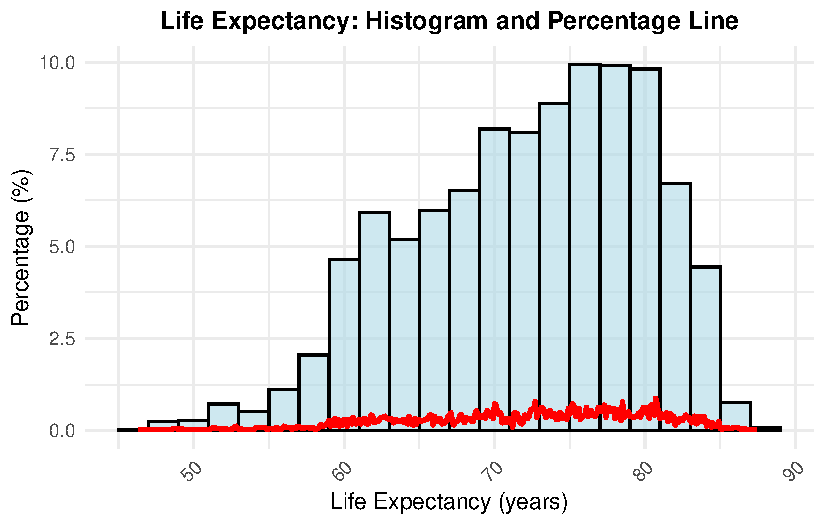
\includegraphics{paper_files/figure-pdf/fig-expectancy-1.pdf}

}

\caption{\label{fig-expectancy}This histogram shows the distribution of
the percentage of life expectancy for all years. Among all the life
expectancy ranges, 76-81 has the largest percenage of 24.7\%, while the
46-51 has the 0.54\%. Life expectancy shows a growing trend with the
increasing of age and drop sharply comes to the 81-86 range.}

\end{figure}%

\subsection{Predictor Variables}\label{predictor-variables}

The \textbf{predictor variables} (or independent variables) are the
factors believed to influence the life expectancy:

\begin{enumerate}
\def\labelenumi{\arabic{enumi}.}
\item
  \textbf{Income Group(\texttt{Income\_Group})}: The income group of a
  country is the key factor influencing the life expectancy. This
  variable provides context for comparing life expectancy between
  different levels of country income group. The division of the life
  expectancy by the income group of a country because income levels
  often correlate strongly with various factors affecting health and
  longevity. Higher income countries typically have more resources to
  invest in robust healthcare systems, with better living conditions
  while lower income countries often face challenges such as inadequate
  healthcare infrastructure and malnutrition. Following by the four
  income group, we would like to see the distribution of the income
  group of 184 WHO member countries. Figure~\ref{fig-income} shows that
  there are 55 countries at the high income group, 26 countries at low
  income group, 54 countries at the lower-middle group while there are
  49 countries at the upper-middle group. With significant less low
  income countries, we expect to see the life expectancy lie in a
  comparably higher range. On the other hand, there might exist sever
  outliers dropping the mean.
\item
  \textbf{Gender(\texttt{Gender})}: The gender of the population of each
  country is included as a categorical variable (Male/Female/Both Sex).
  This is a key variable in the dataset because gender has been fully
  recognized connected with the biological physical factor which
  directly effect the life expectancy. Figure~\ref{fig-gender} shows
  that the with an stable average of 74, life expectancy of female is
  constantly higher than male's average of 70. The line plot reveals a
  steady increase until 2019, followed by a sharp decline in 2020, which
  is assumed to be associated with the impact of COVID-19.
\item
  \textbf{Region(Region)}: This is a categorical variable that
  classifies the geographic location of the countries. It is mapped one
  by one by the name of the country. The data is stored as the name of
  the continent(`Africa', `Oceania', `Asia', `Europe', `North America',
  `South America'). Figure~\ref{fig-region} indicates that with the
  number of 54, Africa has the most WHO member countries. Both Asia and
  Europe has 43 countries,listing in the middle while the other three
  continent has the significant less number of countries. North America
  has 22 countries, South America has 12 countries and Oceania has the
  least, 10 countries.
\end{enumerate}

\begin{figure}

\centering{

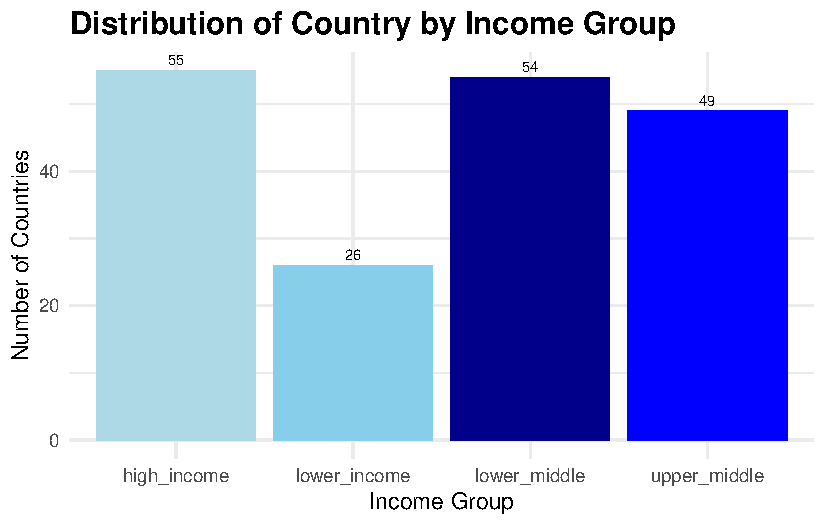
\includegraphics{paper_files/figure-pdf/fig-income-1.pdf}

}

\caption{\label{fig-income}Distribution of country income group. Among
184 WHO member countries, there are 55 high income countries, 54 lower
middle income countries and 49 upper middle income countries. There are
significant less lower income countries, which we could assume there
might exist less outliers in life experctanncy.}

\end{figure}%

\begin{figure}

\centering{

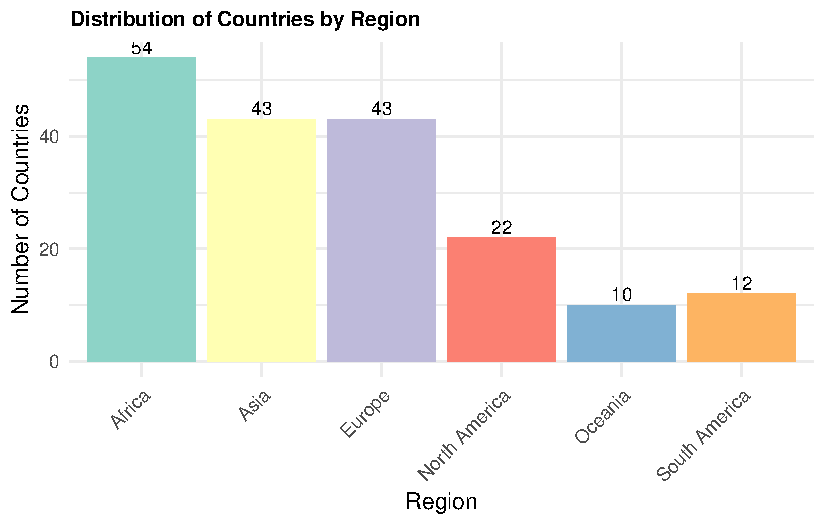
\includegraphics{paper_files/figure-pdf/fig-region-1.pdf}

}

\caption{\label{fig-region}Distribution of different region of the 184
countries. Africa has the most countries with an number of 54. Asia and
Europe has the same amount of 43, North America has 22 countries while
the other two continent has almost the same amount of countries.}

\end{figure}%

\begin{figure}

\centering{

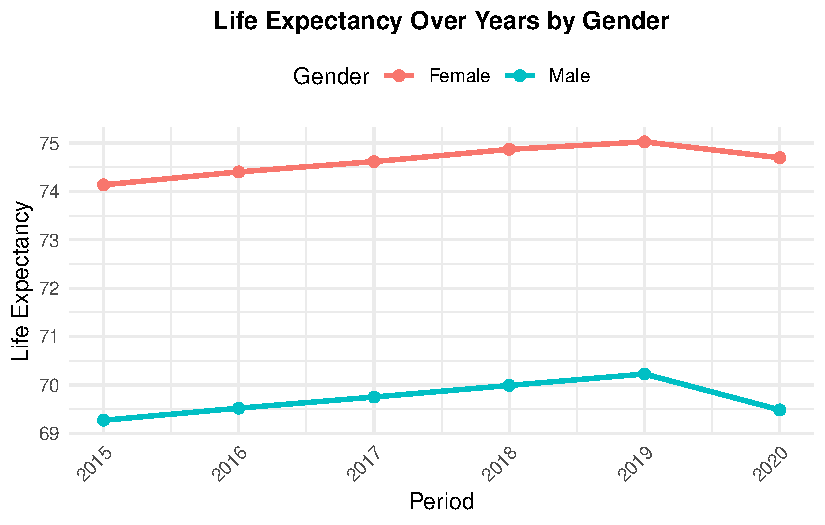
\includegraphics{paper_files/figure-pdf/fig-gender-1.pdf}

}

\caption{\label{fig-gender}Distribution of gender each year. The average
of female life expectancy is approximately 74 around years, constantly
higher than male's average of 70. Compared to male, female's life
expectancy is marginally more steady.}

\end{figure}%

\subsection{Basic Data Summary}\label{basic-data-summary}

The table below shows the basic summary of the mean, median, max,
standard deviation, variance and sample size of life expectancy. We
could tell that the average of the life expectancy from the 6 years is
72.2, with a relatively small standard deviation of 7.8. The max of the
life expectancy is 87.4, among all 3312 rows of data. The variance is
high because of the range of data is large, in other words, because the
mean and median are 72.2 and 73.1, compared to the max 87.4, there is
likely some outliers in the data creating such a slightly high variance
of 60.1.

\begin{figure}

\centering{

\begingroup\fontsize{14}{16}\selectfont

\begin{longtable*}[t]{cccccc}
\toprule
Mean & Median & Max & Standard Deviation & Variance & N\\
\midrule
72.2 & 73.1 & 87.4 & 7.8 & 60.1 & 3312\\
\bottomrule
\end{longtable*}
\endgroup{}

}

\caption{\label{fig-summary}Summary statistics of the number of life
expectancy over countries and years. Less difference between mean and
median, showing that the life expectancy distribution might shows a
naturally bell curve.However, variance is slightly high indicates that
the tails on both sides might be long.}

\end{figure}%

\section{Model}\label{model}

\subsection{Model set-up}\label{sec-modset}

The goal of the Bayesian model is to incorporate prior knowledge, such
as insights from previous studies or analyses, into the selection of the
model. To predict the outcome of the life expectancy of people from
different regions, in this paper, we developed a linear regression
models using R (R Core Team 2023). The outcome variable,
\textbf{\texttt{Life\ Expectancy}}, is a continuous and represents the
average number of years a person is expected to live, assuming all
related resources remain constant throughout their lifetime. The model
aim to estimate and predict the life expectancy of people under
different gender, region and income group. The normal Gaussian
distribution is effective when used for modeling scenarios where the
residuals of the data are assumed to be independent nd normally
distributed around the regression line. The GAM allows for capturing
potential non-linear relationships between the predictors and the
outcome.

The model is specified as follows:

\begin{align*} 
y_i|\mu_i, \sigma &\sim \text{Normal}(\mu_i, \sigma) \\
\mu_i &= \alpha + \beta_1 \text{Region}_i + \beta_2 \text{Gender}_i + \beta_3 \text{Income\_Group}_i \\
\alpha &\sim \text{Normal}(0, 2.5) \\
\beta_1, \beta_2, \beta_3 &\sim \text{Normal}(0, 2.5) \\
\sigma &\sim \text{Exponential}
\end{align*}

Where:

\begin{itemize}
\item
  \(yi\) is the outcome variable (Life Expectancy)for the i-th
  observation.
\item
  \(\mu_i\): the linear predictor for life expectancy, including the
  intercept (\(\alpha\)) and the coefficients for the predictors Region,
  Country, Income Group, and Gender.
\item
  Priors for the intercept(\(\alpha\)) and the
  coefficients(\(\beta_1, \beta_2, \beta_3\)) are normal with mean 0 and
  standard deviation 2.5
\item
  \(\sigma\): the residual standard deviation, modeled as an exponential
  distribution with rate 1.
\end{itemize}

We run the model in R (R Core Team 2023) using the \texttt{rstanarm}
package of Goodrich et al. (2020). We use the default priors from
\texttt{rstanarm}. More explanation of the model could be found
Appendix~\ref{sec-model-details}.

\subsection{Model justification}\label{sec-modjust}

The linear regression model with Gaussian likelihood was chosen for this
analysis due to its simplicity and effectiveness in modeling continuous
outcome variables, such as life expectancy. Life expectancy is
influenced by multiple factors, including region, income group, and
gender. The linear model allows us to examine the average effect of each
predictor on the outcome, assuming that the relationships between these
predictors and life expectancy are linear.

The use of normal priors for the model coefficients \(\alpha\) and
\(\beta\) reflects a belief in prior knowledge that the true values of
these parameters are centered around zero, with some uncertainty, which
is consistent with standard Bayesian modeling practices. The prior scale
of 2.5 was chosen to reflect a reasonable level of uncertainty around
the estimates without being overly restrictive.

The Gaussian distribution was selected because life expectancy data, by
nature, is continuous and expected to follow a normal distribution. The
assumption of normal residuals is consistent with the idea that
deviations from the regression line are random and normally distributed,
allowing the model to make accurate inferences about the relationship
between predictors and the outcome.

Additionally, the exponential prior on the standard deviation \(\alpha\)
captures the residual variability in life expectancy across countries
and regions. The exponential distribution was chosen because it provides
a simple and interpretable way of modeling the variability, assuming
that the data are not heavily skewed.

This approach is appropriate given the data structure and the goal of
the analysis, which is to estimate and predict life expectancy across
different countries, regions, income groups, and genders. The model's
assumptions about the data, along with its priors, allow for robust
inference in the context of population health predictions.

\subsection{Model Validation}\label{model-validation}

To assess the performance of the life expectancy prediction model, two
critical metrics were used: Root Mean Squared Error (RMSE) and
Out-of-Sample Testing. These methods help ensure that the model
generalizes well to unseen data and provides reliable predictions for
life expectancy across different regions, income groups, and genders.

RMSE measures the square root of the average squared differences between
the predicted and observed values. In the context of this model, RMSE
quantifies how closely the predicted life expectancy values align with
the actual observed values. Lower RMSE values indicate better model
performance, suggesting that the model's predictions are close to the
true values. Table~\ref{tbl-modelpredict} gives out the RMSE of both
testing data and training data. The generalizability is checked by
comparing rmse\_test and rmse\_train. Seeing the test RMSE is slightly
lower than the training RMSE, the model generalizes well.

Out-of-Sample testing is a critical component of model evaluation. In
this approach, the data is split into a training set and a test set (or
holdout set). The training set is used to fit the model, while the test
set is used to evaluate how well the model performs on new, unseen data.
For this analysis, the model was trained using a portion of the data
(80\% of the dataset) and then evaluated on the remaining data (20\% of
the dataset) that was not used during training. This method allows us to
check whether the model overfits the training data or if it can
generalize well to unseen observations.

Together, RMSE and out-of-sample testing offer a robust framework for
model validation, ensuring that the predictions made by the life
expectancy model are both accurate and generalizable.

Extended versions of the table can be found in
Table~\ref{tbl-testpredicted}.

\begingroup\fontsize{14}{16}\selectfont

\begin{longtable}[t]{cc}

\caption{\label{tbl-modelpredict}Summary of the life expectancy model,
which includes gender, region and income group. The table presents the
model RSME and out-of sample testing. Seeing the testing data slightly
less than the training data, our model is under good generalization.}

\tabularnewline

\toprule
Dataset & RMSE\\
\midrule
Test Data & 1.15\\
Training Data & 1.17\\
\bottomrule

\end{longtable}

\endgroup{}

\section{Results}\label{sec-result}

\subsection{Data results analysis}\label{data-results-analysis}

According to Figure~\ref{fig-summary}, we could tell that the mean life
expectancy over the 6 years is 72.2, with a relatively low standard
deviation of 7.8. This suggests that, on average, life expectancy across
the dataset is fairly consistent, with only moderate variation from the
mean. However, the maximum life expectancy of 87.4 stands out
significantly, indicating that some countries or regions are achieving
substantially higher life expectancy.With the mean at 72.2 and the
median at 73.1, it's apparent that the data is fairly symmetric, with
the median being slightly higher than the mean, suggesting a mild left
skew. This shift, combined with the large maximum value, hints at the
presence of outliers---countries with exceptionally high life expectancy
that pull the maximum up. The variance of 60.1 is relatively large,
further supporting the idea that the data spans a wide range, with some
observations considerably deviating from the central tendency.

Given this, the high variance can be attributed to the diversity in life
expectancy values across different regions, particularly when countries
at the higher end of the spectrum (e.g., those with life expectancy
around 87 years) are compared with those at the lower end. This
variability suggests that while most countries have life expectancy near
72 years, the outliers significantly influence the spread of the data,
leading to a higher variance than what would be expected in a more
homogenous dataset. Therefore, while the standard deviation is
relatively small, the data is far from uniform, and a deeper analysis of
the outliers could provide further insights into the factors
contributing to the high life expectancy in certain regions.

Table~\ref{tbl-sum_sta} summarizes global life expectancy across various
categories such as gender, geographic regions, and income levels. We
could tell that the global life expectancy is 72.13 years, providing a
benchmark against which other categories can be compared. Women have a
significantly higher life expectancy (74.62 years) than men (69.71
years), which reflects a common global trend due to biological and
social factors. Region variation does happens to influence the life
expectncy. Europe has the highest life expectancy (78.50 years), which
is likely due to better healthcare and living conditions, with having
the most amount of high income countries. Africa has the lowest (64.17
years), potentially reflecting challenges like limited healthcare
infrastructure, poverty, and infectious diseases. Income level, as one
of the most essential factor, significantly affect the life expectancy.
High-income countries have the highest life expectancy (79.38 years),
illustrating the correlation between economic wealth and longevity. High
income level are believed to enable better living standard compared to
other income groups. Upper middle income countries has an average of
73.38 years, where we could observe that the difference is significant
lower than high income group. Lower middle income group has the life
expectancy drop to 68.40. While these countries usually face challenges
such as infrastructure and limit access to health resources, economic
growth may need to be taken seriously be policy makers. Lower-income
countries have a significantly lower life expectancy of 62.35 years,
which can be attributed to limited access to healthcare, education, and
basic services. Table~\ref{tbl-sum_sta} highlights global inequalities
and emphasizes the importance of improving living standards, especially
in lower-income and underdeveloped regions.

\subsection{Overview of model results}\label{overview-of-model-results}

Our results are summarized in Table~\ref{tbl-model}. We are primarily
interest in the general life expectancy regarding to the related
predictors. The multiple linear model provides us with the estimates for
the intercept and coefficients for the predictors which are male,
female, both genders, lower income, lower-middle, upper-middle, high
income, Asia, Europe, Africa, Oceania, North America and South America.
The intercept represents the estimate of region-standard life expectancy
when all the predictors are zero. The coefficients represent the
additional life expectancy associated with each predictor. The model
results will display the estimates- posterior means or medians for each
coefficient including the intercept, uncertainty measures- credible
intervals. The output values of each predictor is the regression
coefficient, meaning how much the outcome is expected to increase or
decrease with one unit increase in the life expectancy (per year) of
that predictor, holding all else constant. The value in the brackets
represent the Median Absolute Deviation of the posterior distributions
of the coefficients. It conveys the dispersion around the median of each
coefficients' posterior distribution, exhibiting how spread the
distributions are.

Num.Obs represents the number of observations made in the model. R2 is
the R-squared value which is the proportion of variance in the dependent
variable that can be explained bu the independent variable. The R2 adj
is the adjusted R squared which accounts for the number of predictors
used. Log.lik is the log-likelihood which gives us an idea of the
likelihood of the data, higher is the better, but this is typically used
for comparison between the models. ELPD and ELPD s.e. explains the log
predictive density and its standard error. The ELPD measures the sum of
the log predictive densities for each observation, used for model
comparison. LOOIC is an acronym for leave-one-out information criterion
in which a lower value indicates a model with better out-of-sample
predictive performance. WAIC stands for Watanabe-Akaike information
criterion which is another measure of good fit; lower values are better
fit. RMSE is the room mean squared error measuring the models's
predictive performance where lower values means more accurate predicts.

\begin{table}

\caption{\label{tbl-model}Summary of the life expectancy model, which
includes gender, region and income group. The table presents the model
RSME and out-of sample testing.}

\centering{

\centering\centering
\fontsize{7.5}{9.5}\selectfont
\begin{tabular}[t]{lc}
\toprule
  & Gaussian(Normal)\\
\midrule
(Intercept) & \num{79.53}\\
 & (\num{43.50})\\
RegionAsia & \num{-6.22}\\
 & \vphantom{1} (\num{21.20})\\
RegionEurope & \num{-8.39}\\
 & (\num{45.65})\\
RegionNorth America & \num{-5.48}\\
 & (\num{50.68})\\
RegionOceania & \num{-8.43}\\
 & (\num{80.66})\\
RegionSouth America & \num{21.91}\\
 & (\num{55.21})\\
CountryAlbania & \num{0.68}\\
 & (\num{28.99})\\
CountryAlgeria & \num{9.41}\\
 & (\num{47.74})\\
CountryAngola & \num{-4.60}\\
 & \vphantom{2} (\num{47.88})\\
CountryAntigua and Barbuda & \num{2.12}\\
 & (\num{31.15})\\
CountryArgentina & \num{-28.26}\\
 & (\num{65.45})\\
CountryArmenia & \num{-3.20}\\
 & (\num{29.08})\\
CountryAustralia & \num{17.28}\\
 & (\num{64.59})\\
CountryAustria & \num{7.63}\\
 & \vphantom{1} (\num{26.97})\\
CountryAzerbaijan & \num{-2.97}\\
 & (\num{29.29})\\
CountryBahamas & \num{-1.15}\\
 & (\num{31.29})\\
CountryBahrain & \num{3.35}\\
 & (\num{36.83})\\
CountryBangladesh & \num{4.23}\\
 & (\num{54.21})\\
CountryBarbados & \num{2.55}\\
 & (\num{30.97})\\
CountryBelarus & \num{-3.11}\\
 & (\num{29.12})\\
CountryBelgium & \num{7.36}\\
 & (\num{26.87})\\
CountryBelize & \num{0.25}\\
 & (\num{30.40})\\
CountryBenin & \num{-3.17}\\
 & \vphantom{1} (\num{48.20})\\
CountryBhutan & \num{4.36}\\
 & (\num{54.23})\\
CountryBolivia (Plurinational State of) & \num{-24.08}\\
 & (\num{76.01})\\
CountryBosnia and Herzegovina & \num{-0.20}\\
 & (\num{29.18})\\
CountryBotswana & \num{-19.85}\\
 & (\num{51.26})\\
CountryBrazil & \num{-30.04}\\
 & (\num{65.42})\\
CountryBrunei Darussalam & \num{4.00}\\
 & (\num{36.91})\\
CountryBulgaria & \num{-2.45}\\
 & (\num{29.09})\\
CountryBurkina Faso & \num{-5.08}\\
 & (\num{21.33})\\
CountryBurundi & \num{-3.23}\\
 & (\num{21.40})\\
CountryCabo Verde & \num{7.65}\\
 & (\num{47.94})\\
CountryCambodia & \num{-0.02}\\
 & \vphantom{1} (\num{54.13})\\
CountryCameroon & \num{-5.86}\\
 & (\num{48.02})\\
CountryCanada & \num{7.86}\\
 & (\num{30.96})\\
CountryCentral African Republic & \num{-14.92}\\
 & \vphantom{1} (\num{21.25})\\
CountryChad & \num{-8.32}\\
 & (\num{21.18})\\
CountryChile & \num{-24.65}\\
 & (\num{56.84})\\
CountryChina & \num{-4.35}\\
 & \vphantom{2} (\num{51.31})\\
CountryColombia & \num{-27.30}\\
 & (\num{65.38})\\
CountryComoros & \num{1.26}\\
 & (\num{48.11})\\
CountryCongo & \num{-3.93}\\
 & (\num{48.00})\\
CountryCosta Rica & \num{5.85}\\
 & (\num{30.49})\\
CountryCote d'Ivoire & \num{-4.15}\\
 & (\num{48.20})\\
CountryCroatia & \num{4.47}\\
 & \vphantom{3} (\num{26.98})\\
CountryCuba & \num{3.41}\\
 & (\num{30.53})\\
CountryCyprus & \num{8.31}\\
 & (\num{26.83})\\
CountryCzechia & \num{5.01}\\
 & \vphantom{1} (\num{27.04})\\
CountryDemocratic People's Republic of Korea & \num{11.23}\\
 & (\num{0.48})\\
CountryDemocratic Republic of the Congo & \num{-5.91}\\
 & \vphantom{1} (\num{21.28})\\
CountryDenmark & \num{7.40}\\
 & \vphantom{1} (\num{26.95})\\
CountryDjibouti & \num{-1.98}\\
 & (\num{47.97})\\
CountryDominican Republic & \num{-0.78}\\
 & \vphantom{1} (\num{30.48})\\
CountryEcuador & \num{-28.26}\\
 & (\num{65.51})\\
CountryEgypt & \num{4.21}\\
 & (\num{47.84})\\
CountryEl Salvador & \num{-0.99}\\
 & (\num{30.48})\\
CountryEquatorial Guinea & \num{-22.60}\\
 & (\num{51.41})\\
CountryEritrea & \num{-3.74}\\
 & (\num{21.28})\\
CountryEstonia & \num{4.46}\\
 & \vphantom{1} (\num{26.91})\\
CountryEswatini & \num{-12.28}\\
 & \vphantom{1} (\num{48.03})\\
CountryEthiopia & \num{1.13}\\
 & \vphantom{1} (\num{21.26})\\
CountryFiji & \num{-0.68}\\
 & (\num{71.02})\\
CountryFinland & \num{7.61}\\
 & (\num{27.08})\\
CountryFrance & \num{8.48}\\
 & \vphantom{2} (\num{26.98})\\
CountryGabon & \num{-19.19}\\
 & (\num{51.46})\\
CountryGambia & \num{-2.56}\\
 & (\num{21.32})\\
CountryGeorgia & \num{-3.87}\\
 & \vphantom{1} (\num{29.20})\\
CountryGermany & \num{7.02}\\
 & \vphantom{2} (\num{27.00})\\
CountryGhana & \num{-1.35}\\
 & (\num{47.86})\\
CountryGreece & \num{7.16}\\
 & \vphantom{1} (\num{26.98})\\
CountryGrenada & \num{-1.25}\\
 & \vphantom{1} (\num{30.43})\\
CountryGuatemala & \num{-2.17}\\
 & (\num{30.39})\\
CountryGuinea & \num{-6.20}\\
 & \vphantom{1} (\num{47.88})\\
CountryGuinea-Bissau & \num{-8.80}\\
 & \vphantom{1} (\num{21.23})\\
CountryGuyana & \num{-37.07}\\
 & (\num{56.78})\\
CountryHaiti & \num{-1.41}\\
 & (\num{33.25})\\
CountryHonduras & \num{6.26}\\
 & (\num{33.17})\\
CountryHungary & \num{2.27}\\
 & \vphantom{1} (\num{27.02})\\
CountryIceland & \num{8.69}\\
 & \vphantom{2} (\num{26.93})\\
CountryIndia & \num{1.11}\\
 & \vphantom{1} (\num{54.41})\\
CountryIndonesia & \num{-10.63}\\
 & \vphantom{1} (\num{51.36})\\
CountryIran (Islamic Republic of) & \num{7.86}\\
 & (\num{54.06})\\
CountryIraq & \num{-9.81}\\
 & (\num{51.25})\\
CountryIreland & \num{8.03}\\
 & \vphantom{1} (\num{26.93})\\
CountryIsrael & \num{9.91}\\
 & \vphantom{1} (\num{36.89})\\
CountryItaly & \num{8.81}\\
 & (\num{26.91})\\
CountryJamaica & \num{-1.99}\\
 & (\num{30.43})\\
CountryJapan & \num{11.94}\\
 & (\num{36.88})\\
CountryJordan & \num{9.67}\\
 & (\num{54.24})\\
CountryKazakhstan & \num{-4.71}\\
 & (\num{29.26})\\
CountryKenya & \num{-0.86}\\
 & (\num{47.87})\\
CountryKiribati & \num{4.08}\\
 & (\num{61.70})\\
CountryKuwait & \num{9.87}\\
 & (\num{36.84})\\
CountryKyrgyzstan & \num{3.47}\\
 & (\num{54.41})\\
CountryLao People's Democratic Republic & \num{-1.48}\\
 & (\num{54.13})\\
CountryLatvia & \num{1.45}\\
 & (\num{26.95})\\
CountryLebanon & \num{9.14}\\
 & (\num{54.11})\\
CountryLesotho & \num{-15.82}\\
 & \vphantom{1} (\num{48.08})\\
CountryLiberia & \num{-4.50}\\
 & (\num{21.35})\\
CountryLibya & \num{-10.87}\\
 & \vphantom{1} (\num{51.31})\\
CountryLithuania & \num{1.52}\\
 & (\num{27.02})\\
CountryLuxembourg & \num{9.05}\\
 & (\num{26.98})\\
CountryMadagascar & \num{-3.54}\\
 & \vphantom{2} (\num{21.21})\\
CountryMalawi & \num{-4.38}\\
 & (\num{21.25})\\
CountryMalaysia & \num{-6.51}\\
 & \vphantom{1} (\num{51.20})\\
CountryMaldives & \num{-4.14}\\
 & (\num{51.20})\\
CountryMali & \num{-6.00}\\
 & \vphantom{1} (\num{21.21})\\
CountryMalta & \num{8.28}\\
 & (\num{26.88})\\
CountryMauritania & \num{2.98}\\
 & \vphantom{1} (\num{47.95})\\
CountryMauritius & \num{-9.94}\\
 & (\num{51.30})\\
CountryMexico & \num{0.67}\\
 & (\num{30.33})\\
CountryMicronesia (Federated States of) & \num{8.09}\\
 & (\num{61.64})\\
CountryMongolia & \num{1.06}\\
 & (\num{54.16})\\
CountryMontenegro & \num{-0.28}\\
 & (\num{29.22})\\
CountryMorocco & \num{6.69}\\
 & (\num{48.03})\\
CountryMozambique & \num{-9.56}\\
 & (\num{21.26})\\
CountryMyanmar & \num{-0.94}\\
 & \vphantom{1} (\num{54.36})\\
CountryNamibia & \num{-21.00}\\
 & (\num{51.42})\\
CountryNepal & \num{1.41}\\
 & (\num{54.14})\\
CountryNetherlands (Kingdom of the) & \num{8.02}\\
 & (\num{27.04})\\
CountryNew Zealand & \num{16.32}\\
 & (\num{64.57})\\
CountryNicaragua & \num{13.32}\\
 & (\num{33.40})\\
CountryNiger & \num{-6.88}\\
 & (\num{21.20})\\
CountryNigeria & \num{-4.28}\\
 & (\num{48.05})\\
CountryNorth Macedonia & \num{-1.40}\\
 & (\num{29.34})\\
CountryNorway & \num{8.78}\\
 & (\num{26.93})\\
CountryOman & \num{2.38}\\
 & \vphantom{1} (\num{36.87})\\
CountryPakistan & \num{-3.13}\\
 & (\num{54.28})\\
CountryPanama & \num{4.48}\\
 & (\num{31.13})\\
CountryPapua New Guinea & \num{8.94}\\
 & \vphantom{1} (\num{61.59})\\
CountryParaguay & \num{-29.48}\\
 & (\num{65.36})\\
CountryPeru & \num{-26.42}\\
 & (\num{65.46})\\
CountryPhilippines & \num{0.30}\\
 & (\num{54.15})\\
CountryPoland & \num{3.67}\\
 & \vphantom{1} (\num{27.01})\\
CountryPortugal & \num{7.36}\\
 & (\num{27.07})\\
CountryPuerto Rico & \num{6.28}\\
 & (\num{31.19})\\
CountryQatar & \num{5.93}\\
 & (\num{36.80})\\
CountryRepublic of Korea & \num{10.61}\\
 & (\num{36.81})\\
CountryRepublic of Moldova & \num{-4.72}\\
 & (\num{29.13})\\
CountryRomania & \num{1.39}\\
 & (\num{26.96})\\
CountryRussian Federation & \num{-9.31}\\
 & (\num{51.36})\\
CountryRwanda & \num{0.44}\\
 & \vphantom{1} (\num{21.29})\\
CountrySaint Lucia & \num{1.72}\\
 & (\num{30.45})\\
CountrySaint Vincent and the Grenadines & \num{-1.25}\\
 & (\num{30.38})\\
CountrySamoa & \num{12.64}\\
 & (\num{61.59})\\
CountrySao Tome and Principe & \num{4.58}\\
 & (\num{47.96})\\
CountrySaudi Arabia & \num{4.35}\\
 & (\num{36.87})\\
CountrySenegal & \num{1.47}\\
 & (\num{48.01})\\
CountrySerbia & \num{-1.59}\\
 & (\num{29.20})\\
CountrySeychelles & \num{-5.53}\\
 & (\num{43.56})\\
CountrySierra Leone & \num{-7.75}\\
 & (\num{21.34})\\
CountrySingapore & \num{10.98}\\
 & (\num{36.89})\\
CountrySlovakia & \num{3.40}\\
 & \vphantom{1} (\num{27.00})\\
CountrySlovenia & \num{7.13}\\
 & (\num{27.00})\\
CountrySolomon Islands & \num{7.87}\\
 & (\num{61.68})\\
CountrySomalia & \num{-12.52}\\
 & (\num{21.30})\\
CountrySouth Africa & \num{-19.37}\\
 & (\num{51.43})\\
CountrySouth Sudan & \num{-8.01}\\
 & (\num{21.29})\\
CountrySpain & \num{8.85}\\
 & (\num{27.13})\\
CountrySri Lanka & \num{7.99}\\
 & (\num{54.25})\\
CountrySudan & \num{1.81}\\
 & (\num{21.31})\\
CountrySuriname & \num{-31.76}\\
 & (\num{65.41})\\
CountrySweden & \num{8.42}\\
 & (\num{26.97})\\
CountrySwitzerland & \num{9.33}\\
 & (\num{27.01})\\
CountrySyrian Arab Republic & \num{3.97}\\
 & \vphantom{1} (\num{0.40})\\
CountryTajikistan & \num{3.09}\\
 & (\num{53.97})\\
CountryThailand & \num{-4.50}\\
 & (\num{51.28})\\
CountryTimor-Leste & \num{-0.90}\\
 & (\num{54.22})\\
CountryTogo & \num{-4.19}\\
 & (\num{21.21})\\
CountryTonga & \num{4.42}\\
 & (\num{71.06})\\
CountryTrinidad and Tobago & \num{0.20}\\
 & (\num{31.16})\\
CountryTunisia & \num{10.40}\\
 & (\num{47.95})\\
CountryTürkiye & \num{-4.47}\\
 & (\num{51.31})\\
CountryTurkmenistan & \num{-12.58}\\
 & (\num{51.24})\\
CountryUganda & \num{-1.74}\\
 & (\num{21.23})\\
CountryUkraine & \num{6.68}\\
 & (\num{36.36})\\
CountryUnited Arab Emirates & \num{8.68}\\
 & (\num{36.79})\\
CountryUnited Kingdom of Great Britain and Northern Ireland & \num{7.08}\\
 & (\num{27.10})\\
CountryUnited Republic of Tanzania & \num{-0.45}\\
 & (\num{47.88})\\
CountryUnited States of America & \num{4.57}\\
 & (\num{31.22})\\
CountryUruguay & \num{-27.80}\\
 & (\num{56.83})\\
CountryUzbekistan & \num{1.65}\\
 & (\num{54.36})\\
CountryVanuatu & \num{9.66}\\
 & (\num{61.72})\\
CountryVenezuela (Bolivarian Republic of) & \num{-31.90}\\
 & (\num{65.65})\\
CountryViet Nam & \num{3.94}\\
 & (\num{53.92})\\
CountryYemen & \num{6.61}\\
 & (\num{0.40})\\
CountryZambia & \num{-5.46}\\
 & (\num{47.98})\\
CountryZimbabwe & \num{-8.25}\\
 & (\num{48.08})\\
Income\_Grouplower\_income & \num{-12.06}\\
 & (\num{36.90})\\
Income\_Grouplower\_middle & \num{-4.04}\\
 & (\num{23.94})\\
Income\_Groupupper\_middle & \num{3.40}\\
 & (\num{20.47})\\
GenderFemale & \num{2.50}\\
 & \vphantom{1} (\num{0.05})\\
GenderMale & \num{-2.42}\\
 & (\num{0.05})\\
\midrule
Num.Obs. & \num{3312}\\
R2 & \num{0.976}\\
R2 Adj. & \num{0.975}\\
Log.Lik. & \num{-5231.038}\\
ELPD & \num{-5409.7}\\
ELPD s.e. & \num{94.5}\\
LOOIC & \num{10819.4}\\
LOOIC s.e. & \num{189.0}\\
WAIC & \num{10816.6}\\
RMSE & \num{4.37}\\
\bottomrule
\end{tabular}

}

\end{table}%

\subsection{Multiple linear regression
results}\label{multiple-linear-regression-results}

Table~\ref{tbl-model} is the table of the results from out model. The
intercept serves as the baseline, which in this case is 79.53. Asia
shows a negative coefficient of -6.22, indicating lower values compared
to the baseline, with a relatively large standard error of 21.20. This
suggests that as the predictor increases, the outcome tends to increase.
In contrast, a negative coefficient implies a decrease in the outcome.
Europe exhibits a negligible negative effect of -8.39, though it also
has a large standard error of 45.65. The effect for females is more
substantial, with a positive coefficient of 2.50 and a standard error of
0.05, indicating considerable variability in the estimate. The male and
lower-middle-income groups show minimal negative coefficients,
suggesting slight decreases from the baseline. The upper-middle-income
group, however, shows a positive effect of 3.40 relative to the
baseline. Regions like North America, Oceania, Asia, and Europe all have
notable negative coefficients, highlighting significant regional
variations. In general, there is a downward trend in coefficients across
countries. Most countries exhibit large standard errors, with European
countries such as Ireland, Israel, and Italy showing slightly positive
trends.

With an R-squared value of 0.976, the model demonstrates a strong level
of explanatory power, supporting the accuracy of the results. The
adjusted R-squared value is 0.975, which is nearly identical to the
R-squared value, indicating the model's robustness with 3,312
observations. The RMSE of 4.37 reflects the average magnitude of the
model's prediction errors, suggesting good predictive accuracy. Although
values like LOOIC and WAIC are excluded due to the lack of alternative
models for comparison, the overall results indicate that the model
performs well on the cleaned dataset.Further evaluation of the model
results will be done in Section~\ref{sec-model-details}.

\section{Discussion}\label{sec-discussion}

\subsection{Insights into Life Expectancy Differences by
Gender}\label{insights-into-life-expectancy-differences-by-gender}

Thought the result part we have noticed that female constantly have
higher life expectancy than male. Figure~\ref{fig-gender} shows that
female has around 4 years higher average age than male. Even during the
sudden drop of 2020, female kept a more stable trend than male. Through
literature research, we found that historically women tend to have
longer life than men across most regions and cultures. (Kalben
2000)These difference can be attributed to a variety of interconnected
reasons. Women generally have stronger immune systems and are less prone
to certain life-threatening diseases like cardiovascular diseases in
early adulthood. Estrogen, a hormone prevalent in women, provides some
protection against heart disease by improving cholesterol levels. On the
other hand, men are more prone to risk factors such as hypertension and
higher levels of LDL cholesterol, which contribute to shorter life
spansehavioral patterns (Oksuzyan 2008a). What's more, male are more
likely to engage in behaviours such as smoking, excessive alcohol
consumption and hazardous occupations. These behaviors increase the risk
of accidents, chronic diseases, and early mortality. Last but not least,
globally, women tend to use healthcare services more frequently than
men, which allows for earlier detection and treatment of illnesses. Men
often delay seeking medical care, worsening outcomes for preventable or
manageable diseases.(Saltonstall 1993)

\subsection{Insights into Life Expectancy Differences by Income
Group}\label{insights-into-life-expectancy-differences-by-income-group}

From the summary and analysis of Table~\ref{tbl-sum_sta}, we have seen
that high income group has the significant high life expectancy compared
to the lower income group, which indicates that life expectancy is
significantly influenced by income groups. It is known that income
determines access to resources, healthcare and living conditions.
Difference in life expectancy across income groups reflect broader
inequalities in socioeconomic factors and highlight disparities in
global health outcomes.

High-income groups have greater access to quality healthcare services,
including preventive care, advanced medical treatments, and regular
health checkups.Conversely, lower-income groups often face barriers such
as cost, lack of infrastructure, and insufficient health insurance
coverage, leading to untreated or poorly managed health conditions (M.
Marmot 2015). Other living conditions like access to nutritious food,
safe drinking water and sanitary living environments are also linked
with high economics. Low-income populations are more likely to
experience malnutrition, exposure to environmental toxins, and
overcrowded living conditions, all of which negatively impact health and
life expectancy.

What's more, lower-income individuals are often exposed to higher levels
of chronic stress due to financial instability and job insecurity.
Stress is linked to adverse health outcomes such as hypertension,
cardiovascular diseases, and mental health issues (Public Health. 2020).
Moreover, low-income workers frequently engage in physically demanding
or hazardous jobs, increasing their risk of injury and illness. All
these factors together makes the lower income countries disadvantage in
life expectancy.

\subsection{Life Expectancy at 60}\label{life-expectancy-at-60}

The life expectancy at 60 means that how long is a person expected to
live at 60 instead of at birth. From the box plot
Figure~\ref{fig-lea60}, we could tell the high-income group tends to
have an average life expectancy of approximately 23 years at age 60,
whereas the lower-income group averages around 16 years. Notably, the
lower-middle-income group exhibits the largest variance, with the most
outliers, indicating a wide disparity in life expectancy within this
category.

The data also reveal a clear trend: as income levels increase, so does
the average life expectancy at age 60. This aligns with findings from
analyses of life expectancy at birth, emphasizing the significant
correlation between income and life expectancy. Higher-income groups
likely benefit from better access to healthcare, nutrition, and living
conditions, which collectively contribute to improved longevity.

Life expectancy at 60 provides insights into the additional years a
person can expect to live after reaching 60, reflecting the health and
living conditions of older populations. Unlike life expectancy at birth,
which captures the average years a newborn is expected to live based on
current mortality rates across all ages, life expectancy at 60 excludes
the impact of child and early-adult mortality. This makes it
particularly useful for assessing health outcomes, chronic disease
management, and the effectiveness of healthcare systems for aging
populations. It highlights longevity and quality of life in later years,
crucial for designing age-focused policies and support systems.

\begin{figure}

\centering{

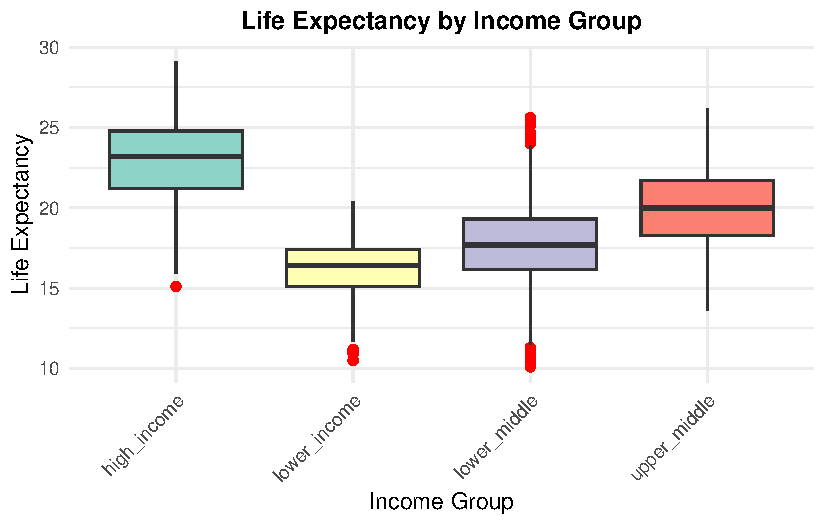
\includegraphics{paper_files/figure-pdf/fig-lea60-1.pdf}

}

\caption{\label{fig-lea60}Box plot of life expectancy at 60 by different
income group. The high income group tend to have 23 years of life
expectancy at 60 while the lower income group has an average of 16 years
at 60. It is noticable that lower middle has the most outlier showing
the largest varaiance.}

\end{figure}%

\subsection{Weaknesses and next steps}\label{weaknesses-and-next-steps}

\subsubsection{Other factors related to income group and
region}\label{other-factors-related-to-income-group-and-region}

Income groups, often categorized as low, middle, or high-income, play a
significant role in determining access to resources and opportunities
that directly and indirectly affect life expectancy. However, income
group classifications themselves are shaped by a variety of factors that
this analysis may not have accounted for, which introduces limitations
to the model. Region would be one key factor that influence the income
group. Regions with limited access to stable employment opportunities
may fall into lower-income groups, leading to reduced access to
healthcare, education, and nutritious food, all of which affect life
expectancy. It is reckon that trade imbalances, resource exploitation,
and historical colonization have left some countries with weak economies
and infrastructure, directly influencing their classification as low or
middle-income. Since these factors influence the income groups, their
absence in the model creates a gap in understanding how income
ultimately impacts life expectancy. A comprehensive model should explore
these underlying determinants of income groups alongside traditional
predictors of life expectancy.

\subsubsection{Dataset limitation}\label{dataset-limitation}

Weakness may arise from the generalization of the data. When working
with data provided by authoritative sources like the World Health
Organization (WHO), it's important to recognize the methodological
nuances underlying the calculations. In this case, the dataset includes
average life expectancy values, which are themselves estimates derived
from sophisticated statistical and demographic models. The accuracy of
the derived averages depends heavily on the statistical methods used by
WHO. Since the initial dataset offers the average of the life expectancy
of each country which are calculated after several factor, these
assumptions cascade into our analysis. The ``average of averages''
cannot rectify inaccuracies or gaps in the original model.

By acknowledging these limitations and incorporating appropriate
statistical techniques, for further studies, it would be suggested to
use a more variety of models such as the multilevel modeling to increase
the accuracy of the model by cross validation or comparing the results
from other models as well. Study deeper into the correlations with more
factors we discussed above would let us notice which factors influences
life expectancy. Like mentioned in the introduction, this analysis aims
to empower policymakers by providing critical insights into factors
affecting life expectancy across various regions, genders, and income
groups. By addressing identified limitations and leveraging data-driven
strategies, analyses can better capture the complexities of life
expectancy data and provide insights that align more closely with
real-world dynamics while policymakers can implement targeted
interventions to improve healthcare access, reduce disparities, and
enhance the overall quality of life for their populations.

\newpage

\appendix

\section{Appendix}\label{sec-appx}

\subsection{Data Cleaning Notes}\label{data-cleaning-notes}

We began by importing the raw dataset using the read\_csv function from
the tidyverse package. To focus our analysis on more relevant variables,
we selected specific columns, such as Indicator of life expectancy as
birth and life expectancy at 60 years, Country, Period, Gender, and Life
expectancy, omitting any unnecessary columns.

We functioned to extract the number before opening the square bracket of
life expectancy since the raw data gave both the range and the mean of
life expectancy of each country under each year.

We filter out the rows containing NA values in any of the selected
columns for reducing the noise and simpler further analysis.

We then renaming columns for clarity. For example, we changed `Location'
into `Country', ``Dim1'' for ``Gender'' and ``Value'' for ``Life
Expectancy'', making it easier for anyone working with the data to read
and understand what each variable represents.

Each column is rounded using the round function, specifying the desired
number of decimal places for each. Columns not mentioned in mutate
remain unchanged. This ensures a flexible and precise cleaning process
tailored to further comparison and graphing. We dropped the potential
percentage symbol to contain purely numerical data.

The income group column and the region column was not given in the raw
dataset. We created a new variable called ``Income\_Group'' by mapping
over country name to four income group (``lower\_income'',
``lower\_middle'', ``upper\_middle'', ``high\_income'') according to the
index given by World Bank Income Group. This is a key variable in
predicting life expectancy since it is believed that life expectancy is
correlated to the income situation. We as well made a mapping to the
countries according to its continent and saved as ``Region''. This is
the variable indicates the geographic context to the analysis. Countries
are mapped into six continents (``Africa'', ``Asia'', ``Europe'',
``North America'', ``South America'', ``Oceania'') one by one.

We again merge the table, removing repeated columns and rows and mapping
the region and the country income under different given names.

Lastly, we filter out NAs again as a further check. We continue filter
out the Palestinian territory, which is not a country and was not mapped
in neither Region nor Income Group.

For easy reading format, we arrange the country into Alphabet order and
mutate the variables again for converting columns into appropriate data
types.

For easier visualization, we created four tables, which are grouped by
life expectancy at age 60, life expectancy at birth, life expectancy at
birth of Male and life expectancy at birth of Female.

After completing the cleaning, we saved the final dataset in both
Parquet and CSV formats for later analysis.

\subsection{Data Cleaning Table}\label{data-cleaning-table}

\begingroup\fontsize{5.5}{7.5}\selectfont

\begin{longtable}[t]{llll}

\caption{\label{tbl-cleaned_average}Cleaned data of average life
expectancy of 6 years by different countries.}

\tabularnewline

\toprule
Country & Income Group & Region & Average Life Expectancy\\
\midrule
Afghanistan & lower\_income & Asia & 60.63\\
Albania & upper\_middle & Europe & 77.65\\
Algeria & lower\_middle & Africa & 75.95\\
Angola & lower\_middle & Africa & 62.13\\
Antigua and Barbuda & high\_income & North America & 75.93\\
\addlinespace
Argentina & upper\_middle & South America & 76.55\\
Armenia & upper\_middle & Europe & 74.08\\
Australia & high\_income & Oceania & 82.77\\
Austria & high\_income & Europe & 81.32\\
Azerbaijan & upper\_middle & Europe & 74.08\\
\addlinespace
Bahamas & high\_income & North America & 72.62\\
Bahrain & high\_income & Asia & 75.67\\
Bangladesh & lower\_middle & Asia & 73.48\\
Barbados & high\_income & North America & 76.35\\
Belarus & upper\_middle & Europe & 73.98\\
\addlinespace
Belgium & high\_income & Europe & 81.10\\
Belize & upper\_middle & North America & 74.58\\
Benin & lower\_middle & Africa & 63.52\\
Bhutan & lower\_middle & Asia & 73.68\\
Bolivia (Plurinational State of) & lower\_middle & South America & 71.53\\
\addlinespace
Bosnia and Herzegovina & upper\_middle & Europe & 76.90\\
Botswana & upper\_middle & Africa & 63.93\\
Brazil & upper\_middle & South America & 74.87\\
Brunei Darussalam & high\_income & Asia & 76.55\\
Bulgaria & upper\_middle & Europe & 74.58\\
\addlinespace
Burkina Faso & lower\_income & Africa & 62.02\\
Burundi & lower\_income & Africa & 63.75\\
Cabo Verde & lower\_middle & Africa & 74.38\\
Cambodia & lower\_middle & Asia & 69.25\\
Cameroon & lower\_middle & Africa & 60.83\\
\addlinespace
Canada & high\_income & North America & 81.67\\
Central African Republic & lower\_income & Africa & 51.98\\
Chad & lower\_income & Africa & 58.72\\
Chile & high\_income & South America & 80.53\\
China & upper\_middle & Asia & 77.00\\
\addlinespace
Colombia & upper\_middle & South America & 77.45\\
Comoros & lower\_middle & Africa & 67.92\\
Congo & lower\_middle & Africa & 62.80\\
Costa Rica & upper\_middle & North America & 80.25\\
Cote d'Ivoire & lower\_middle & Africa & 62.42\\
\addlinespace
Croatia & high\_income & Europe & 78.13\\
Cuba & upper\_middle & North America & 77.82\\
Cyprus & high\_income & Europe & 81.97\\
Czechia & high\_income & Europe & 78.73\\
Democratic People's Republic of Korea & lower\_income & Asia & 71.95\\
\addlinespace
Democratic Republic of the Congo & lower\_income & Africa & 61.07\\
Denmark & high\_income & Europe & 80.95\\
Djibouti & lower\_middle & Africa & 64.78\\
Dominican Republic & upper\_middle & North America & 73.50\\
Ecuador & upper\_middle & South America & 76.62\\
\addlinespace
Egypt & lower\_middle & Africa & 70.87\\
El Salvador & upper\_middle & North America & 73.52\\
Equatorial Guinea & upper\_middle & Africa & 61.20\\
Eritrea & lower\_income & Africa & 63.28\\
Estonia & high\_income & Europe & 78.22\\
\addlinespace
Eswatini & lower\_middle & Africa & 54.23\\
Ethiopia & lower\_income & Africa & 68.15\\
Fiji & upper\_middle & Oceania & 67.82\\
Finland & high\_income & Europe & 81.35\\
France & high\_income & Europe & 82.17\\
\addlinespace
Gabon & upper\_middle & Africa & 64.60\\
Gambia & lower\_income & Africa & 64.42\\
Georgia & upper\_middle & Europe & 73.30\\
Germany & high\_income & Europe & 80.72\\
Ghana & lower\_middle & Africa & 65.30\\
\addlinespace
Greece & high\_income & Europe & 80.73\\
Grenada & upper\_middle & North America & 73.08\\
Guatemala & upper\_middle & North America & 72.22\\
Guinea & lower\_middle & Africa & 60.38\\
Guinea-Bissau & lower\_income & Africa & 58.33\\
\addlinespace
Guyana & high\_income & South America & 67.85\\
Haiti & lower\_middle & North America & 63.18\\
Honduras & lower\_middle & North America & 70.82\\
Hungary & high\_income & Europe & 75.97\\
Iceland & high\_income & Europe & 82.35\\
\addlinespace
India & lower\_middle & Asia & 70.10\\
Indonesia & upper\_middle & Asia & 70.77\\
Iran (Islamic Republic of) & lower\_middle & Asia & 77.15\\
Iraq & upper\_middle & Asia & 71.68\\
Ireland & high\_income & Europe & 81.57\\
\addlinespace
Israel & high\_income & Asia & 82.35\\
Italy & high\_income & Europe & 82.55\\
Jamaica & upper\_middle & North America & 72.37\\
Japan & high\_income & Asia & 84.35\\
Jordan & lower\_middle & Asia & 78.90\\
\addlinespace
Kazakhstan & upper\_middle & Europe & 72.52\\
Kenya & lower\_middle & Africa & 65.72\\
Kiribati & lower\_middle & Oceania & 61.67\\
Kuwait & high\_income & Asia & 81.78\\
Kyrgyzstan & lower\_middle & Asia & 72.57\\
\addlinespace
Lao People's Democratic Republic & lower\_middle & Asia & 67.85\\
Latvia & high\_income & Europe & 75.18\\
Lebanon & lower\_middle & Asia & 78.77\\
Lesotho & lower\_middle & Africa & 50.85\\
Liberia & lower\_income & Africa & 62.53\\
\addlinespace
Libya & upper\_middle & Africa & 73.02\\
Lithuania & high\_income & Europe & 75.25\\
Luxembourg & high\_income & Europe & 82.68\\
Madagascar & lower\_income & Africa & 63.52\\
Malawi & lower\_income & Africa & 62.70\\
\addlinespace
Malaysia & upper\_middle & Asia & 74.85\\
Maldives & upper\_middle & Asia & 77.25\\
Mali & lower\_income & Africa & 61.05\\
Malta & high\_income & Europe & 82.02\\
Mauritania & lower\_middle & Africa & 69.68\\
\addlinespace
Mauritius & upper\_middle & Africa & 74.02\\
Mexico & upper\_middle & North America & 75.03\\
Micronesia (Federated States of) & lower\_middle & Oceania & 65.65\\
Mongolia & lower\_middle & Asia & 70.48\\
Montenegro & upper\_middle & Europe & 76.77\\
\addlinespace
Morocco & lower\_middle & Africa & 73.33\\
Mozambique & lower\_income & Africa & 57.47\\
Myanmar & lower\_middle & Asia & 68.27\\
Namibia & upper\_middle & Africa & 62.75\\
Nepal & lower\_middle & Asia & 70.78\\
\addlinespace
Netherlands (Kingdom of the) & high\_income & Europe & 81.62\\
New Zealand & high\_income & Oceania & 81.72\\
Nicaragua & lower\_middle & North America & 77.85\\
Niger & lower\_income & Africa & 60.17\\
Nigeria & lower\_middle & Africa & 62.45\\
\addlinespace
North Macedonia & upper\_middle & Europe & 75.65\\
Norway & high\_income & Europe & 82.38\\
Oman & high\_income & Asia & 74.30\\
Pakistan & lower\_middle & Asia & 66.28\\
Panama & high\_income & North America & 78.27\\
\addlinespace
Papua New Guinea & lower\_middle & Oceania & 66.35\\
Paraguay & upper\_middle & South America & 75.15\\
Peru & upper\_middle & South America & 78.33\\
Philippines & lower\_middle & Asia & 69.50\\
Poland & high\_income & Europe & 77.38\\
\addlinespace
Portugal & high\_income & Europe & 81.03\\
Puerto Rico & high\_income & North America & 80.03\\
Qatar & high\_income & Asia & 78.22\\
Republic of Korea & high\_income & Asia & 83.15\\
Republic of Moldova & upper\_middle & Europe & 72.35\\
\addlinespace
Romania & high\_income & Europe & 74.97\\
Russian Federation & upper\_middle & Asia & 72.12\\
Rwanda & lower\_income & Africa & 67.55\\
Saint Lucia & upper\_middle & North America & 76.08\\
Saint Vincent and the Grenadines & upper\_middle & North America & 72.98\\
\addlinespace
Samoa & lower\_middle & Oceania & 70.03\\
Sao Tome and Principe & lower\_middle & Africa & 71.20\\
Saudi Arabia & high\_income & Asia & 76.70\\
Senegal & lower\_middle & Africa & 68.18\\
Serbia & upper\_middle & Europe & 75.47\\
\addlinespace
Seychelles & high\_income & Africa & 73.82\\
Sierra Leone & lower\_income & Africa & 59.28\\
Singapore & high\_income & Asia & 83.43\\
Slovakia & high\_income & Europe & 77.10\\
Slovenia & high\_income & Europe & 80.78\\
\addlinespace
Solomon Islands & lower\_middle & Oceania & 65.43\\
Somalia & lower\_income & Africa & 54.43\\
South Africa & upper\_middle & Africa & 64.55\\
South Sudan & lower\_income & Africa & 59.03\\
Spain & high\_income & Europe & 82.58\\
\addlinespace
Sri Lanka & lower\_middle & Asia & 77.58\\
Sudan & lower\_income & Africa & 68.85\\
Suriname & upper\_middle & South America & 73.03\\
Sweden & high\_income & Europe & 82.13\\
Switzerland & high\_income & Europe & 83.07\\
\addlinespace
Syrian Arab Republic & lower\_income & Asia & 64.13\\
Tajikistan & lower\_middle & Asia & 72.70\\
Thailand & upper\_middle & Asia & 76.95\\
Timor-Leste & lower\_middle & Asia & 68.32\\
Togo & lower\_income & Africa & 62.77\\
\addlinespace
Tonga & upper\_middle & Oceania & 72.78\\
Trinidad and Tobago & high\_income & North America & 73.98\\
Tunisia & lower\_middle & Africa & 77.08\\
Türkiye & upper\_middle & Asia & 76.98\\
Turkmenistan & upper\_middle & Asia & 68.92\\
\addlinespace
Uganda & lower\_income & Africa & 65.37\\
Ukraine & lower\_middle & Europe & 72.65\\
United Arab Emirates & high\_income & Asia & 80.85\\
United Kingdom of Great Britain and Northern Ireland & high\_income & Europe & 80.72\\
United Republic of Tanzania & lower\_middle & Africa & 66.23\\
\addlinespace
United States of America & high\_income & North America & 78.32\\
Uruguay & high\_income & South America & 77.17\\
Uzbekistan & lower\_middle & Asia & 70.83\\
Vanuatu & lower\_middle & Oceania & 66.98\\
Venezuela (Bolivarian Republic of) & upper\_middle & South America & 72.87\\
\addlinespace
Viet Nam & lower\_middle & Asia & 73.62\\
Yemen & lower\_income & Asia & 67.25\\
Zambia & lower\_middle & Africa & 61.28\\
Zimbabwe & lower\_middle & Africa & 58.47\\
\bottomrule

\end{longtable}

\endgroup{}

\subsection{Idealized Survey}\label{idealized-survey}

\textbf{Survey: Life Expectancy and Lifestyle Survey}

Thank you for participating in this survey. This survey aims to gather
insights into the factors influencing life expectancy, including gender,
region and income group. Your responses will help us understand
individual perspectives and experience towards national policy.
Participation is voluntary, and your answers will remain anonymous.

\textbf{Contact Information:} If you have any questions about the survey
or the data collection process, please contact

\textbf{Survey Coordinator}: Yanfei Huang\\
\textbf{Email}: yanfei.huang@mail.utoronto.ca

\textbf{Section 1: Demographics}

\textbf{1. Gender}

\begin{itemize}
\tightlist
\item
  Male
\item
  Female
\item
  Non-binary
\item
  Prefer not to say
\end{itemize}

\textbf{2. Age (in years)}

Please write the number: \_\_\_\_\_\_

\textbf{3. Region of Residence}

\begin{itemize}
\tightlist
\item
  Africa
\item
  Asia
\item
  Europe
\item
  North America
\item
  South America
\item
  Oceania
\end{itemize}

\textbf{4. Income Level}

Annual Income (Optional): \_\_\_\_\_\_ USD

Income Group: - Low Income (Less than \$1,000/year) - Lower-Middle
Income (\$1,001 - \$10,000/year) - Upper-Middle Income (\$10,001 -
\$50,000/year) - High Income (More than \$50,000/year)

\textbf{Section 2: Health and Lifestyle}

\textbf{5. Current Life Expectancy Perception}

How many years do you expect to live?

Please write the number: \_\_\_\_\_\_

\textbf{6. Healthcare Access}

How often do you visit healthcare professionals - Regularly (e.g.,
annual checkups) - Occasionally (e.g., only when unwell) - Rarely or
Never

\textbf{7. Dietary Habits}

How would you describe your diet?

\begin{itemize}
\tightlist
\item
  Balanced and healthy
\item
  Somewhat balanced
\item
  Unhealthy
\end{itemize}

\textbf{8. Physical Activity}

How many hours of physical activity do you engage in per week? - Less
than 1 hour - 1-3 hours - More than 3 hours

\textbf{9. Smoking Habits}

Do you smoke?

\begin{itemize}
\tightlist
\item
  Yes
\item
  No
\end{itemize}

\textbf{10. Alcohol Consumption}

How often do you consume alcoholic beverages?

\begin{itemize}
\tightlist
\item
  Never
\item
  Occasionally (e.g., social drinking)
\item
  Frequently
\end{itemize}

\textbf{Section 3: Environmental and Social Factors}

\textbf{11.Living Environment}

How would you describe your living area?

\begin{itemize}
\tightlist
\item
  Urban
\item
  Suburban
\item
  Rural
\end{itemize}

\textbf{Final Section}

Thank you for completing this survey! Your responses will help capture
information about economic conditions, access to healthcare and
education, and basic living standards, which are critical for
understanding life expectancy predictors and the impact of socioeconomic
factors on health outcomes.

\section{Additional data details}\label{additional-data-details}

\subsection{Model details}\label{sec-model-details}

The model developed for predicting life expectancy is a linear
regression model, where the goal is to estimate the outcome variable,
Life Expectancy, based on multiple predictors: Region, Income Group, and
Gender. Here's a more detailed breakdown of the components and structure
of the model:

\textbf{1. Outcome variable (}\(y_i\))

The outcome variable \(y_i\) represents the life expectancy of an
country. This is a continuous variable representing the number of years
a person is expected to live, assuming all conditions remain constant.

\textbf{2. Linear Predictor (}\(μ_i\))

The linear predictor \(μ_i\) is a linear combination of the predictors,
which includes an intercept term \(α\) and the coefficients \(β_1\),
\(β_2\), \(β_3\), corresponding to Region, Income Group, and Gender,
respectively. This linear equation models the relationship between life
expectancy and the predictors
\(\mu_i = \alpha + \beta_1(Region) + \beta_2(Income Group) + \beta_3 (Gender)\).
The values for these coefficients (betas) represent the expected change
in life expectancy for a one-unit change in each respective predictor.

\textbf{3. Priors}

The prior distribution for the intercept \(α\) and the coefficients
\(β_1\), \(β_2\), \(β_3\) is assumed to be normal with a mean of 0 and a
standard deviation of 2.5. This reflects our belief that, prior to
seeing the data, the intercept and coefficients are most likely close to
0, with a reasonable range of variability (the scale of 2.5 is
relatively broad, allowing flexibility in fitting the model).

The prior for \(σ\) (residual standard deviation) is assumed to follow
an exponential distribution with a rate of 1. This prior reflects the
assumption that the variance of the residuals (i.e., the deviation of
the actual observations from the predicted values) is positive and that
it could reasonably be spread across a wide range of values.

\textbf{4. Residual Standard Deviation (}\(σ\)) The model also estimates
\(σ\), which represents the standard deviation of the residuals --- the
errors between the observed life expectancy values and those predicted
by the model. The prior for \(σ\) is assumed to follow an exponential
distribution with a rate of 1, meaning that smaller values of \(σ\)
(indicating less variation) are somewhat more likely than larger ones.

\textbf{5. Gaussian Likelihood} The outcome variable Life Expectancy is
modeled using a normal distribution with mean μi (the linear predictor)
and standard deviation σ. This means that the residuals (the differences
between the observed and predicted values) are assumed to be normally
distributed: \(y_i| \mu_i, \sigma ~ Normal(\mu_i, \sigma)\) This is a
typical assumption in regression models when the data is continuous, and
the relationship between the predictors and the outcome is linear.

\subsection{RMSE Full table}\label{rmse-full-table}

\begingroup\fontsize{8.5}{10.5}\selectfont

\begin{longtable}[t]{>{\raggedright\arraybackslash}p{0.35in}r>{\raggedleft\arraybackslash}p{1in}>{\raggedleft\arraybackslash}p{1in}>{\raggedleft\arraybackslash}p{1in}>{\raggedright\arraybackslash}p{1in}}

\caption{\label{tbl-testpredicted}Partical table of the test and
training RMSE of Life expectancy over countries and gender of average of
6 years (First 100 rows). Through the model part we could tell that with
comparing the training and testing data, the model is well generated
without doubt.}

\tabularnewline

\toprule
Country & Actual Life Expectancy & Predicted Life Expectancy & RMSE (Test) & RMSE (Train) & Indication\\
\midrule
Afghanistan & 59.3 & 58.23 & 1.15 & 1.17 & Model generalizes well (out-of-sample)\\
Afghanistan & 61.7 & 63.15 & 1.15 & 1.17 & Model generalizes well (out-of-sample)\\
Afghanistan & 62.1 & 63.15 & 1.15 & 1.17 & Model generalizes well \vphantom{1} (out-of-sample)\\
Afghanistan & 62.1 & 63.15 & 1.15 & 1.17 & Model generalizes well (out-of-sample)\\
Albania & 74.3 & 75.27 & 1.15 & 1.17 & Model generalizes well (out-of-sample)\\
\addlinespace
Albania & 76.2 & 75.27 & 1.15 & 1.17 & Model generalizes well (out-of-sample)\\
Albania & 79.9 & 80.19 & 1.15 & 1.17 & Model generalizes well \vphantom{2} (out-of-sample)\\
Albania & 79.9 & 80.19 & 1.15 & 1.17 & Model generalizes well \vphantom{1} (out-of-sample)\\
Albania & 79.9 & 80.19 & 1.15 & 1.17 & Model generalizes well (out-of-sample)\\
Algeria & 76.1 & 73.58 & 1.15 & 1.17 & Model generalizes well (out-of-sample)\\
\addlinespace
Algeria & 76.0 & 73.58 & 1.15 & 1.17 & Model generalizes well (out-of-sample)\\
Algeria & 75.9 & 73.58 & 1.15 & 1.17 & Model generalizes well (out-of-sample)\\
Angola & 60.3 & 59.70 & 1.15 & 1.17 & Model generalizes well (out-of-sample)\\
Angola & 60.1 & 59.70 & 1.15 & 1.17 & Model generalizes well (out-of-sample)\\
Angola & 64.5 & 64.62 & 1.15 & 1.17 & Model generalizes well (out-of-sample)\\
\addlinespace
Angola & 59.8 & 59.70 & 1.15 & 1.17 & Model generalizes well (out-of-sample)\\
Angola & 61.8 & 62.12 & 1.15 & 1.17 & Model generalizes well (out-of-sample)\\
Antigua and Barbuda & 73.8 & 73.42 & 1.15 & 1.17 & Model generalizes well \vphantom{1} (out-of-sample)\\
Antigua and Barbuda & 75.5 & 75.84 & 1.15 & 1.17 & Model generalizes well (out-of-sample)\\
Antigua and Barbuda & 77.1 & 78.33 & 1.15 & 1.17 & Model generalizes well (out-of-sample)\\
\addlinespace
Antigua and Barbuda & 73.8 & 73.42 & 1.15 & 1.17 & Model generalizes well (out-of-sample)\\
Argentina & 79.9 & 79.01 & 1.15 & 1.17 & Model generalizes well (out-of-sample)\\
Argentina & 76.6 & 76.51 & 1.15 & 1.17 & Model generalizes well (out-of-sample)\\
Argentina & 73.0 & 74.09 & 1.15 & 1.17 & Model generalizes well (out-of-sample)\\
Argentina & 76.1 & 76.51 & 1.15 & 1.17 & Model generalizes well (out-of-sample)\\
\addlinespace
Armenia & 75.7 & 73.90 & 1.15 & 1.17 & Model generalizes well (out-of-sample)\\
Armenia & 79.8 & 76.39 & 1.15 & 1.17 & Model generalizes well (out-of-sample)\\
Armenia & 79.1 & 76.39 & 1.15 & 1.17 & Model generalizes well (out-of-sample)\\
Australia & 82.6 & 82.74 & 1.15 & 1.17 & Model generalizes well (out-of-sample)\\
Australia & 84.2 & 85.24 & 1.15 & 1.17 & Model generalizes well (out-of-sample)\\
\addlinespace
Austria & 81.4 & 81.26 & 1.15 & 1.17 & Model generalizes well \vphantom{1} (out-of-sample)\\
Austria & 83.6 & 83.76 & 1.15 & 1.17 & Model generalizes well (out-of-sample)\\
Austria & 81.4 & 81.26 & 1.15 & 1.17 & Model generalizes well (out-of-sample)\\
Austria & 83.3 & 83.76 & 1.15 & 1.17 & Model generalizes well (out-of-sample)\\
Azerbaijan & 67.5 & 71.62 & 1.15 & 1.17 & Model generalizes well (out-of-sample)\\
\addlinespace
Azerbaijan & 75.8 & 74.04 & 1.15 & 1.17 & Model generalizes well (out-of-sample)\\
Azerbaijan & 72.2 & 71.62 & 1.15 & 1.17 & Model generalizes well (out-of-sample)\\
Azerbaijan & 71.7 & 71.62 & 1.15 & 1.17 & Model generalizes well (out-of-sample)\\
Bahamas & 76.0 & 75.07 & 1.15 & 1.17 & Model generalizes well (out-of-sample)\\
Bahamas & 76.5 & 75.07 & 1.15 & 1.17 & Model generalizes well (out-of-sample)\\
\addlinespace
Bahamas & 73.2 & 72.58 & 1.15 & 1.17 & Model generalizes well (out-of-sample)\\
Bahamas & 69.7 & 70.16 & 1.15 & 1.17 & Model generalizes well (out-of-sample)\\
Bahamas & 72.9 & 72.58 & 1.15 & 1.17 & Model generalizes well (out-of-sample)\\
Bahamas & 76.1 & 75.07 & 1.15 & 1.17 & Model generalizes well (out-of-sample)\\
Bahamas & 69.8 & 70.16 & 1.15 & 1.17 & Model generalizes well (out-of-sample)\\
\addlinespace
Bahrain & 74.9 & 75.74 & 1.15 & 1.17 & Model generalizes well (out-of-sample)\\
Bahrain & 75.9 & 75.74 & 1.15 & 1.17 & Model generalizes well (out-of-sample)\\
Bahrain & 75.7 & 75.74 & 1.15 & 1.17 & Model generalizes well (out-of-sample)\\
Bahrain & 75.8 & 75.74 & 1.15 & 1.17 & Model generalizes well (out-of-sample)\\
Bangladesh & 72.6 & 71.06 & 1.15 & 1.17 & Model generalizes well (out-of-sample)\\
\addlinespace
Bangladesh & 75.0 & 75.97 & 1.15 & 1.17 & Model generalizes well (out-of-sample)\\
Bangladesh & 73.4 & 73.48 & 1.15 & 1.17 & Model generalizes well (out-of-sample)\\
Bangladesh & 73.2 & 73.48 & 1.15 & 1.17 & Model generalizes well (out-of-sample)\\
Barbados & 74.9 & 73.87 & 1.15 & 1.17 & Model generalizes well (out-of-sample)\\
Barbados & 76.3 & 76.30 & 1.15 & 1.17 & Model generalizes well \vphantom{1} (out-of-sample)\\
\addlinespace
Barbados & 77.4 & 78.79 & 1.15 & 1.17 & Model generalizes well (out-of-sample)\\
Barbados & 76.3 & 76.30 & 1.15 & 1.17 & Model generalizes well (out-of-sample)\\
Belarus & 79.7 & 76.42 & 1.15 & 1.17 & Model generalizes well (out-of-sample)\\
Belarus & 79.2 & 76.42 & 1.15 & 1.17 & Model generalizes well (out-of-sample)\\
Belarus & 78.9 & 76.42 & 1.15 & 1.17 & Model generalizes well (out-of-sample)\\
\addlinespace
Belgium & 81.6 & 81.06 & 1.15 & 1.17 & Model generalizes well (out-of-sample)\\
Belize & 74.4 & 74.64 & 1.15 & 1.17 & Model generalizes well (out-of-sample)\\
Benin & 63.7 & 63.54 & 1.15 & 1.17 & Model generalizes well (out-of-sample)\\
Benin & 66.2 & 66.04 & 1.15 & 1.17 & Model generalizes well (out-of-sample)\\
Benin & 65.4 & 66.04 & 1.15 & 1.17 & Model generalizes well (out-of-sample)\\
\addlinespace
Bhutan & 74.5 & 73.70 & 1.15 & 1.17 & Model generalizes well (out-of-sample)\\
Bhutan & 72.3 & 71.28 & 1.15 & 1.17 & Model generalizes well (out-of-sample)\\
Bhutan & 73.3 & 73.70 & 1.15 & 1.17 & Model generalizes well (out-of-sample)\\
Bhutan & 74.2 & 76.19 & 1.15 & 1.17 & Model generalizes well (out-of-sample)\\
Bolivia (Plurinational State of) & 73.8 & 74.04 & 1.15 & 1.17 & Model generalizes well (out-of-sample)\\
\addlinespace
Bolivia (Plurinational State of) & 71.8 & 69.13 & 1.15 & 1.17 & Model generalizes well (out-of-sample)\\
Bolivia (Plurinational State of) & 71.3 & 69.13 & 1.15 & 1.17 & Model generalizes well (out-of-sample)\\
Bolivia (Plurinational State of) & 71.0 & 69.13 & 1.15 & 1.17 & Model generalizes well (out-of-sample)\\
Bolivia (Plurinational State of) & 72.8 & 74.04 & 1.15 & 1.17 & Model generalizes well (out-of-sample)\\
Bosnia and Herzegovina & 74.9 & 74.46 & 1.15 & 1.17 & Model generalizes well (out-of-sample)\\
\addlinespace
Bosnia and Herzegovina & 74.6 & 74.46 & 1.15 & 1.17 & Model generalizes well (out-of-sample)\\
Botswana & 64.9 & 63.88 & 1.15 & 1.17 & Model generalizes well (out-of-sample)\\
Botswana & 64.5 & 63.88 & 1.15 & 1.17 & Model generalizes well (out-of-sample)\\
Botswana & 64.0 & 63.88 & 1.15 & 1.17 & Model generalizes well (out-of-sample)\\
Botswana & 66.1 & 66.37 & 1.15 & 1.17 & Model generalizes well (out-of-sample)\\
\addlinespace
Botswana & 65.0 & 66.37 & 1.15 & 1.17 & Model generalizes well (out-of-sample)\\
Brazil & 75.3 & 74.84 & 1.15 & 1.17 & Model generalizes well (out-of-sample)\\
Brazil & 74.6 & 74.84 & 1.15 & 1.17 & Model generalizes well (out-of-sample)\\
Brunei Darussalam & 78.3 & 79.03 & 1.15 & 1.17 & Model generalizes well (out-of-sample)\\
Brunei Darussalam & 76.4 & 76.54 & 1.15 & 1.17 & Model generalizes well (out-of-sample)\\
\addlinespace
Brunei Darussalam & 77.9 & 79.03 & 1.15 & 1.17 & Model generalizes well (out-of-sample)\\
Bulgaria & 71.4 & 72.17 & 1.15 & 1.17 & Model generalizes well (out-of-sample)\\
Bulgaria & 78.4 & 77.09 & 1.15 & 1.17 & Model generalizes well (out-of-sample)\\
Burkina Faso & 60.3 & 59.54 & 1.15 & 1.17 & Model generalizes well (out-of-sample)\\
Burkina Faso & 62.4 & 61.97 & 1.15 & 1.17 & Model generalizes well (out-of-sample)\\
\addlinespace
Burkina Faso & 58.9 & 59.54 & 1.15 & 1.17 & Model generalizes well (out-of-sample)\\
Burkina Faso & 60.9 & 61.97 & 1.15 & 1.17 & Model generalizes well (out-of-sample)\\
Burundi & 66.2 & 66.23 & 1.15 & 1.17 & Model generalizes well (out-of-sample)\\
Burundi & 63.7 & 63.73 & 1.15 & 1.17 & Model generalizes well (out-of-sample)\\
Burundi & 61.3 & 61.31 & 1.15 & 1.17 & Model generalizes well (out-of-sample)\\
\addlinespace
Burundi & 60.8 & 61.31 & 1.15 & 1.17 & Model generalizes well (out-of-sample)\\
Cabo Verde & 78.2 & 76.82 & 1.15 & 1.17 & Model generalizes well (out-of-sample)\\
Cabo Verde & 69.7 & 71.91 & 1.15 & 1.17 & Model generalizes well (out-of-sample)\\
Cabo Verde & 72.0 & 71.91 & 1.15 & 1.17 & Model generalizes well (out-of-sample)\\
Cabo Verde & 72.2 & 71.91 & 1.15 & 1.17 & Model generalizes well (out-of-sample)\\
\bottomrule

\end{longtable}

\endgroup{}

\newpage

\section*{References}\label{references}
\addcontentsline{toc}{section}{References}

\phantomsection\label{refs}
\begin{CSLReferences}{1}{0}
\bibitem[\citeproctext]{ref-IncomeGroupsandLongevity}
Chetty, Stepner, R. 2016. \emph{The Association Between Income and Life
Expectancy in the United States, 2001-2014}.
\url{https://jamanetwork.com/journals/jama/fullarticle/2513561}.

\bibitem[\citeproctext]{ref-janitor}
Firke, Sam. 2024. \emph{Janitor: Simple Tools for Examining and Cleaning
Dirty Data}. \url{https://github.com/sfirke/janitor}.

\bibitem[\citeproctext]{ref-rstanarm}
Goodrich, Ben, Jonah Gabry, Imad Ali, and Sam Brilleman. 2020.
{``Rstanarm: {Bayesian} Applied Regression Modeling via {Stan}.''}
\url{https://mc-stan.org/rstanarm}.

\bibitem[\citeproctext]{ref-whymandieyounger}
Kalben, B. B. 2000. \emph{Why Men Die Younger: Causes of Mortality
Differences by Sex.}
https://doi.org/\url{https://doi.org/10.1080/10920277.2000.10595939}.

\bibitem[\citeproctext]{ref-ggcorrplot}
Kassambara, Alboukadel. 2029. \emph{Ggcorrplot: Visualization of a
Correlation Matrix Using 'Ggplot2'}.
\url{https://github.com/kassambara/ggcorrplot}.

\bibitem[\citeproctext]{ref-RegionalVariations}
Marmot, Friel, M. 2008. \emph{Closing the Gap in a Generation: Health
Equity Through Action on the Social Determinants of Health.}
\url{chrome-extension://efaidnbmnnnibpcajpcglclefindmkaj/https://iris.who.int/bitstream/handle/10665/43943/9789241563703_eng.pdf}.

\bibitem[\citeproctext]{ref-inequalworld}
Marmot, M. 2015. \emph{The Health Gap: The Challenge of an Unequal
World.} \url{https://doi.org/10.1093/ije/dyx163}.

\bibitem[\citeproctext]{ref-here}
Müller, Kirill. 2023. \emph{Here: A Simpler Way to Find Your Files}.
\url{https://CRAN.R-project.org/package=here}.

\bibitem[\citeproctext]{ref-behaviouralfactor}
Oksuzyan, Juel, A. 2008a. \emph{Behavioral Factors Associated with Life
Expectancy Gaps.}
\url{https://link.springer.com/article/10.1007/BF03324754}.

\bibitem[\citeproctext]{ref-GenderandLifeExpectancy}
---------. 2008b. \emph{Gender and Life Expectancy}.
\url{https://link.springer.com/article/10.1007/BF03324754}.

\bibitem[\citeproctext]{ref-sf}
Pebesma, Edzer, and Roger Bivand. 2023. \emph{{Spatial Data Science:
With applications in R}}. {Chapman and Hall/CRC}.
\url{https://doi.org/10.1201/9780429459016}.

\bibitem[\citeproctext]{ref-incomeinequality}
Public Health., Harvard T. H. Chan School of. 2020. \emph{Income
Inequality and Health Outcomes}.
\url{chrome-extension://efaidnbmnnnibpcajpcglclefindmkaj/https://www.hsph.harvard.edu/horp/wp-content/uploads/sites/94/2020/01/Income-inequality-report-topline_January2020.pdf}.

\bibitem[\citeproctext]{ref-citeR}
R Core Team. 2023. \emph{{R: A Language and Environment for Statistical
Computing}}. Vienna, Austria: R Foundation for Statistical Computing.
\url{https://www.R-project.org/}.

\bibitem[\citeproctext]{ref-arrow}
Richardson, Neal, Ian Cook, Nic Crane, Dewey Dunnington, Romain
François, Jonathan Keane, Dragoș Moldovan-Grünfeld, et al. 2023.
\emph{Arrow: Integration to 'Apache Arrow'}.
\url{https://CRAN.R-project.org/package=arrow}.

\bibitem[\citeproctext]{ref-womenhigherhealthcare}
Saltonstall, R. 1993. \emph{Health and Gender: A Case for Women's Higher
Healthcare Utilization.}
https://doi.org/\url{https://doi.org/10.1016/0277-9536(93)90300-S}.

\bibitem[\citeproctext]{ref-lifeexpectancy}
WHO. 2020. \emph{Life Expectancy}.
\url{https://www.who.int/data/gho/data/indicators/indicator-details/GHO/life-expectancy-at-age-60-(years)}.

\bibitem[\citeproctext]{ref-tidyverse}
Wickham, Hadley, Mara Averick, Jennifer Bryan, Winston Chang, Lucy
D'Agostino McGowan, Romain François, Garrett Grolemund, et al. 2019.
{``Welcome to the {tidyverse}.''} \emph{Journal of Open Source Software}
4 (43): 1686. \url{https://doi.org/10.21105/joss.01686}.

\bibitem[\citeproctext]{ref-ggplot2}
Wickham, Hadley, Winston Chang, Lionel Henry, Thomas Lin Pedersen,
Kohske Takahashi, Claus Wilke, Kara Woo, Hiroaki Yutani, Dewey
Dunnington, and Teun van den Brand. 2023. \emph{Ggplot2: Create Elegant
Data Visualisations Using the Grammar of Graphics}.
\url{https://CRAN.R-project.org/package=ggplot2}.

\bibitem[\citeproctext]{ref-dplyr}
Wickham, Hadley, Romain François, Lionel Henry, Kirill Müller, and Davis
Vaughan. 2023. \emph{Dplyr: A Grammar of Data Manipulation}.
\url{https://CRAN.R-project.org/package=dplyr}.

\bibitem[\citeproctext]{ref-purrr}
Wickham, Hadley, and Lionel Henry. 2023. \emph{Purrr: Functional
Programming Tools}. \url{https://purrr.tidyverse.org/}.

\bibitem[\citeproctext]{ref-socialdeterminantsofhealth}
Wilkinson, \& Marmot, R. G. 2003. \emph{Social Determinants of Health:
The Solid Facts.} \url{https://iris.who.int/handle/10665/326568}.

\bibitem[\citeproctext]{ref-knitr}
Xie, Yihui. 2024. \emph{Knitr: A General-Purpose Package for Dynamic
Report Generation in r}. \url{https://yihui.org/knitr/}.

\bibitem[\citeproctext]{ref-kableExtra}
Zhu, Hao. 2023. \emph{kableExtra: Construct Complex Table with 'Kable'
and Pipe Syntax}. \url{https://CRAN.R-project.org/package=kableExtra}.

\end{CSLReferences}




\end{document}
